\documentclass[nojss]{jss}\usepackage[]{graphicx}\usepackage[]{color}
%% maxwidth is the original width if it is less than linewidth
%% otherwise use linewidth (to make sure the graphics do not exceed the margin)
\makeatletter
\def\maxwidth{ %
  \ifdim\Gin@nat@width>\linewidth
    \linewidth
  \else
    \Gin@nat@width
  \fi
}
\makeatother

\usepackage{Sweave}



%\usepackage{setspace}
% \usepackage[sc]{mathpazo}
\usepackage{amsmath}
% %\usepackage{geometry} 
% %\geometry{verbose, tmargin = 1.25cm, bmargin = 1.25cm, lmargin = 1.25cm, rmargin = 1.25cm}
% \setcounter{secnumdepth}{2}
% \setcounter{tocdepth}{2}
\usepackage{longtable}
\usepackage{colortbl, xcolor}
\usepackage{booktabs}

%%%%%%%%%%%%%%%%%%%%%%%%%%%%%%
%% declarations for jss.cls %%
%%%%%%%%%%%%%%%%%%%%%%%%%%%%%%
%\VignetteEngine{knitr::knitr}
%\VignetteIndexEntry{survivalRandomForest}
%\VignetteIndexEntry{Random Forests for Survival ggRandomForests packages}                     
%\VignetteKeywords{random forest, survival, VIMP, minimal depth}                                  
%\VignetteDepends{ggRandomForests}                   
%\VignettePackage{ggRandomForests} 

%% almost as usual
\author{John Ehrlinger 
\and Eugene H. Blackstone\\Cleveland Clinic}

\title{\pkg{ggRandomForests}: Survival with Random Forests}

%% for pretty printing and a nice hypersummary also set:
\Plainauthor{Ehrlinger et.\ al.} %% comma-separated
\Plaintitle{ggRandomForests: Random Forests for Survival} %% without formatting
\Shorttitle{Random Forests for Survival}

%% an abstract and keywords
\Abstract{ 
Random Forests~\citep{Breiman:2001} (RF) are a fully non-parametric statistical method requiring no distributional assumptions on covariate relation to the response. RF are a robust, nonlinear technique that optimizes predictive accuracy by fitting an ensemble of trees to stabilize model estimates. Random Forests for survival~\citep{Ishwaran:2007a, Ishwaran:2008} (RF-S) are an extension of Breiman's RF techniques to survival settings, allowing efficient non-parametric analysis of time to event data. The \pkg{randomForestSRC} package~\citep{Ishwaran:RFSRC:2014} is a unified treatment of Breiman's random forests for survival, regression and classification problems.

Predictive accuracy make RF an attractive alternative to parametric models, though complexity and interpretability of the forest hinder wider application of the method. We introduce the \pkg{ggRandomForests} package, tools for creating and plotting data structures to visually understand random forest models grown in \proglang{R} with the \pkg{randomForestSRC} package. The \pkg{ggRandomForests} package is structured to extract intermediate data objects from \pkg{randomForestSRC} objects and generate figures using the \pkg{ggplot2}~\citep{Wickham:2009} graphics package.

This document is formatted as a tutorial for using the \pkg{randomForestSRC} for building random forests for survival and \pkg{ggRandomForests} package for investigating how the forest is constructed. This tutorial uses the Primary Biliary Cirrhosis (PBC) Data from the Mayo Clinic~\citep{fleming:1991} available in the \pkg{randomForestSRC} package. We use Variable Importance measure (VIMP)~\citep{Breiman:2001} as well as Minimal Depth~\citep{Ishwaran:2010}, a property derived from the construction of each tree within the forest, to assess the impact of variables on forest prediction. We will also demonstrate the use of variable dependence plots~\citep{Friedman:2000} to aid interpretation RF results in different response settings. We also will investigate interactions between covariates to demonstrate the strength of the Random Forest method in survival settings.
}
\Keywords{random forest, survival, VIMP, minimal depth, \proglang{R}, \pkg{randomForestSRC}}
\Plainkeywords{random forest, survival, VIMP, minimal depth, R, randomForestSRC}
%% at least one keyword must be supplied

%% publication information
%% NOTE: Typically, this can be left commented and will be filled out by the technical editor
%% \Volume{13}
%% \Issue{9}
%% \Month{September}
%% \Year{2004}
%% \Submitdate{2004-09-29}
%% \Acceptdate{2004-09-29}

%% The address of (at least) one author should be given
%% in the following format:
\Address{
John Ehrlinger\\
Quantitative Health Sciences\\
Lerner Research Institute\\
Cleveland Clinic\\
9500 Euclid Ave\\
Cleveland, Ohio 44195\\
% Telephone: + 41/0/44634-4643 \\
% Fax: + 41/0/44634-4386 \\
E-mail: \email{john.ehrlinger@gmail.com}\\
URL: \url{http://www.lerner.ccf.org/qhs/people/ehrlinj/}
}

%% It is also possible to add a telephone and fax number
%% before the e-mail in the following format:
%% Telephone: + 43/1/31336-5053
%% Fax: + 43/1/31336-734

%% for those who use Sweave please include the following line (with % symbols):
%% need no \usepackage{Sweave.sty}

%% end of declarations %%%%%%%%%%%%%%%%%%%%%%%%%%%%%%%%%%%%%%%%%%%%%%%



\IfFileExists{upquote.sty}{\usepackage{upquote}}{}
\begin{document}
% -----------------------------------------------------
\section*{About this document}\addcontentsline{toc}{section}{About this document}
% -----------------------------------------------------

This document is a package vignette for the \pkg{ggRandomForests} (\url{http://CRAN.R-project.org/package = ggRandomForests}) package for ``Visually Exploring Random Forests''. \pkg{ggRandomForests} will help uncover variable associations in random forest models. The package is designed for use with the \pkg{randomForestSRC} (\url{http://CRAN.R-project.org/package = randomForestSRC}) package~\citep{Ishwaran:RFSRC:2014} for survival, regression and classification forests and uses the \pkg{ggplot2}(\url{http://CRAN.R-project.org/package = ggplot2}) package~\citep{Wickham:2009} for plotting diagnostic and variable association results. \pkg{ggRandomForests} is  structured to extract data objects from \pkg{randomForestSRC} objects and provides S3 functions for printing and plotting these objects.

The vignette is a tutorial for using the \pkg{ggRandomForests} package with the \pkg{randomForestSRC} package for building and post-processing a survival random forest. In this tutorial, we explore a random forest for survival model for the primary biliary cirrhosis (PBC) of the liver data set~\citep{fleming:1991}, available in the \pkg{randomForestSRC} package. We grow a survival random forest and demonstrate how \pkg{ggRandomForests} can be used when determining variable associations, interactions and how the survival response depends on predictive variables within the model. The tutorial demonstrates the design and usage of many of \pkg{ggRandomForests} functions and features how to modify and customize the resulting ggplot2 graphic objects along the way.

The latest version of this vignette is available within the \pkg{ggRandomForests} package on the Compreshensive R Archive Network (CRAN) (\url{http://cran.r-project.org}). Once the package has been installed, the vignette can be viewed directly from within \proglang{R} with the following command:
\begin{Schunk}
\begin{Sinput}
R> vignette("randomForestSurvival", package = "ggRandomForests")
\end{Sinput}
\end{Schunk}

A development version of the \pkg{ggRandomForests} package is also available on Github (\url{https://github.com}). We invite comments, feature requests and bug reports for this package at \url{https://github.com/ehrlinger/ggRandomForests}.

% -----------------------------------------------------
\section{Introduction} \label{S:introduction}
% -----------------------------------------------------

Random Forests~\citep{Breiman:2001} (RF) are a fully non-parametric statistical method which requires no distributional assumptions on covariate relation to the response. RF is a robust, nonlinear technique that optimizes predictive accuracy by fitting an ensemble of trees to stabilize model estimates. Random Survival Forests (RSF)~\citep{Ishwaran:2007a,Ishwaran:2008} are an extension of Breiman's RF techniques to survival settings, allowing efficient non-parametric analysis of time to event data. The \pkg{randomForestSRC} (\url{http://CRAN.R-project.org/package = ggRandomForests}) package~\citep{Ishwaran:RFSRC:2014} is a unified treatment of Breiman's random forests for survival, regression and classification problems.

Predictive accuracy make RF an attractive alternative to parametric models, though complexity and interpretability of the forest hinder wider application of the method. We introduce the \pkg{ggRandomForests} (\url{http://CRAN.R-project.org/package = ggRandomForests}) package for visually exploring random forest models. The \pkg{ggRandomForests} package is structured to extract intermediate data objects from \pkg{randomForestSRC} objects and generate figures using the \pkg{ggplot2} (\url{http://CRAN.R-project.org/package = ggplot2}) graphics package~\citep{Wickham:2009}.

Many of the figures created by the \pkg{ggRandomForests} package are also available directly from within the \pkg{randomForestSRC} package. However \pkg{ggRandomForests} offers the following advantages:
\begin{itemize}
\item Separation of data and figures: \pkg{ggRandomForests} contains functions that  operate on either the \code{randomForestSRC::rfsrc} forest object directly, or on the output from \pkg{randomForestSRC} post processing functions (i.e. \code{plot.variable}, \code{var.select}, \code{find.interaction}) to generate intermediate \pkg{ggRandomForests} data objects. S3 functions are provide to further process these objects and plot results using the \pkg{ggplot2} graphics package. Alternatively, users can use these data objects for their own custom plotting or analysis operations.  

\item Each data object/figure is a single, self contained object. This allows simple modification and manipulation of the data or \pkg{ggplot2} objects to meet users specific needs and requirements. 

\item The use of \pkg{ggplot2} for plotting. We chose to use the \pkg{ggplot2} package for our figures to allow users flexibility in modifying the figures to their liking. Each S3 plot function returns either a single \pkg{ggplot2} object, or a \code{list} of \pkg{ggplot2} objects, allowing users to use additional \pkg{ggplot2} functions or themes to modify and customize the figures to their liking.  
\end{itemize}

This document is formatted as a tutorial for using the \pkg{randomForestSRC} package for building and post-processing random survival forest models with the \pkg{ggRandomForests} package for investigating how the forest is constructed. In this tutorial, we will investigate the primary biliary cirrhosis (PBC) of the liver data set~\citep{fleming:1991}, available in the \pkg{randomForestSRC} package. We present the data in Section~\ref{S:data} before building a random survival forest in Section~\ref{S:rfsrcGrow}. 

Random forests are not parsimonious, but use all variables available in the construction of a response predictor. We demonstrate a random forest variable selection process (Section~\ref{S:variableselection}) using the Variable Importance measure (VIMP)~\citep{Breiman:2001} in Section~\ref{S:vimp} as well as Minimal Depth~\citep{Ishwaran:2010} in Section~\ref{S:minimalDepth}. Minimal depth is a property derived from the construction of each tree within the forest, which we use to assess the impact of variables on forest prediction. 

Once we have an idea of which variables the forest is using for prediction, we will use variable dependence plots~\citep{Friedman:2000} (Section~\ref{S:dependence}) to understand how a variable is related to the response. Marginal variable dependence (Section~\ref{S:variabledependence}) plots give us an idea of the overall trend of a variable/response relation, while partial dependence plots (Section~\ref{S:partialdependence}) show us a risk adjusted relation. These figures often show strongly non-linear variable/response relations that are not easily obtained through a parametric approach. We are also interested in examining variable interactions (Section~\ref{S:interactions}) within the forest model. Using a minimal depth approach, we can quantify how closely variables are related within the forest, and generate marginal dependence and partial dependence (risk adjusted) conditioning plots (coplots)~\citep{chambers:1992,cleveland:1993} to examine these interactions graphically  (Section~\ref{S:coplots}).

\section{Data Summary: Primary Biliary Cirrhosis (PBC) Data}\label{S:data}

Data was obtained from a Mayo Clinic randomized trial in primary biliary cirrhosis (PBC) of the liver conducted between 1974 and 1984. A total of 424 PBC patients, referred to Mayo Clinic during that ten year interval met eligibility criteria for the randomized placebo controlled trial of the drug D-penicillamine (DPCA). The data and partial likelihood model is described in~\cite{fleming:1991} in Chapter 0.2 and Chapter 4.4 and is listed in Appendix D. The \code{pbc} data set included in the \pkg{randomForestSRC} package contains 418 observations, with 312 patients participating in the randomized trial.

\begin{Schunk}
\begin{Sinput}
R> data(pbc, package = "randomForestSRC")
\end{Sinput}
\end{Schunk}



We will do some modification of the data for formating our results. Since the data contains about 12 years of follow up, we prefer using \code{years} instead of \code{days} survival. We also convert the \code{age} variable to years, and the \code{treatment} variable to a factor containing levels of \code{c("DPCA", "placebo")}. The variable names, type and description are outlined in Table~\ref{T:dataLabs}.

% latex table generated in R 3.1.2 by xtable 1.7-4 package
% Sun Jan  4 09:53:39 2015
\begin{table}[ht]
\centering
{\footnotesize
\begin{tabular}{rll}
  \toprule
 & label & type \\ 
  \midrule
status & event indicator (F = censor, T = death) & logical \\ 
   \rowcolor[gray]{0.95}treatment & Treament (DPCA, Placebo) & factor \\ 
  age & age in years & numeric \\ 
   \rowcolor[gray]{0.95}sex & Female & logical \\ 
  ascites & Asictes & logical \\ 
   \rowcolor[gray]{0.95}hepatom & Hepatomegaly & logical \\ 
  spiders & Spiders & logical \\ 
   \rowcolor[gray]{0.95}edema & Edema & factor \\ 
  bili & serum bilirubin (mg/dl) & numeric \\ 
   \rowcolor[gray]{0.95}chol & serum cholesterol (mg/dl) & integer \\ 
  albumin & albumin (gm/dl) & numeric \\ 
   \rowcolor[gray]{0.95}copper & urine copper (ug/day) & integer \\ 
  alk & alkaline phosphatase (U/liter) & numeric \\ 
   \rowcolor[gray]{0.95}sgot & SGOT (U/ml) & numeric \\ 
  trig & triglicerides (mg/dl) & integer \\ 
   \rowcolor[gray]{0.95}platelet & platelets per cubic ml/1000 & integer \\ 
  prothrombin & prothrombin time (sec) & numeric \\ 
   \rowcolor[gray]{0.95}stage & histologic stage & factor \\ 
  years & survival time (years) & numeric \\ 
   \rowcolor[gray]{0.95} \bottomrule
\end{tabular}
}
\caption{PBC Data field descriptions} 
\label{T:dataLabs}
\end{table}


\subsection{Exploratory Data Analysis}\label{S:eda}

It is good practice to view your data before beginning an analysis, what~\cite{Tukey:1977} refers to as Exploratory Data Analysis (EDA). To facilitate this, we use \pkg{ggplot2} figures with the \code{facet_wrap} command to create two sets of panel plots, one for categorical variables using histograms (Figure~\ref{fig:categoricalEDA}), and another of scatter plots for continuous variables (Figure~\ref{fig:continuousEDA}). Each variable is plotted along a selected continuous variable on the X-axis, in this case the length of follow up (survival time in \code{years}). These figures help to find outliers, missing values and other data anomalies within each variable before getting deep into the analysis.

\begin{Schunk}
\begin{figure}[!htpb]

{\centering 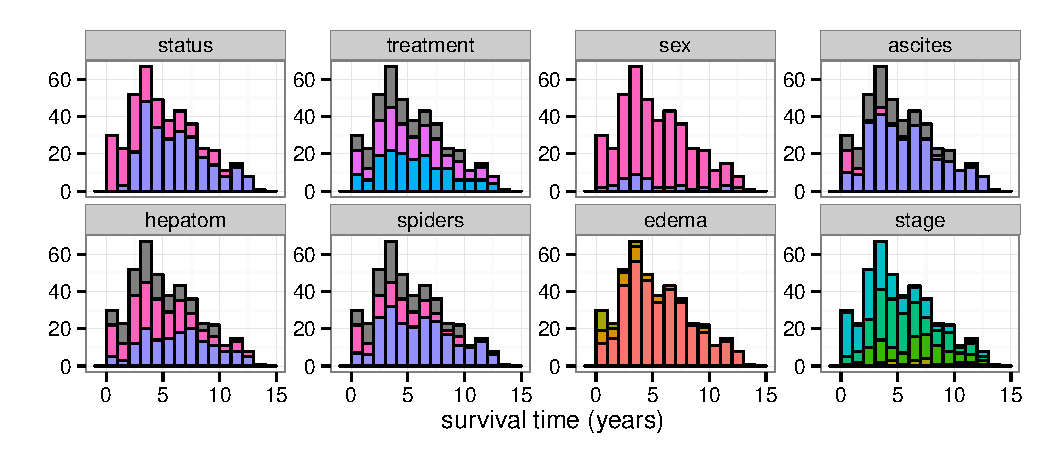
\includegraphics[width=\maxwidth]{figure/rfs-categoricalEDA-1} 

}

\caption[Categorical variable EDA plots]{Categorical variable EDA plots. Bars indicate counts within 1 year of followup for each categorical variable. Bars are colored according to the class membership within each variable. Missing values are colored dark grey.\label{fig:categoricalEDA}}
\end{figure}
\end{Schunk}


\begin{Schunk}
\begin{figure}[!htpb]

{\centering 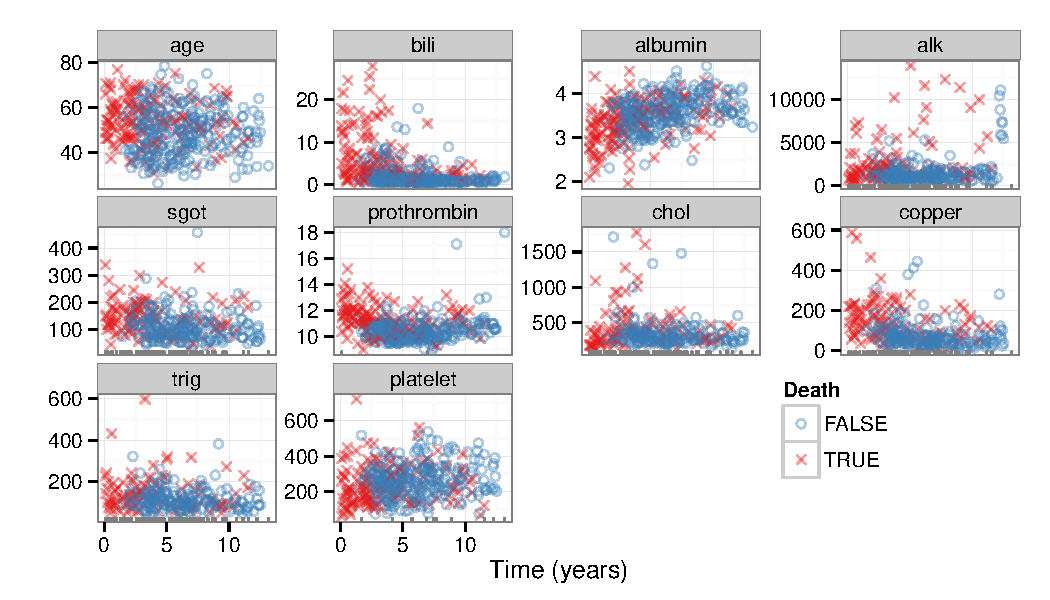
\includegraphics[width=\maxwidth]{figure/rfs-continuousEDA-1} 

}

\caption[Continuous variable EDA plots]{Continuous variable EDA plots. Points indicate variable value against the follow up time in years. Points are colored according to the death event in the  \code{status} variable. Missing values are indicated by the rug marks along the X-axis\label{fig:continuousEDA}}
\end{figure}
\end{Schunk}

In categorical EDA plots (Figure~\ref{fig:categoricalEDA}) we are looking for patterns of missing data. We often use surgical date for our X-axis variable to look for periods of low enrollment. The variable was not available in this data set, so we used follow up time (\code{years}) instead. Another good choice may have been to use the \code{age} variable.

In continuous EDA plots (Figure~\ref{fig:continuousEDA}) we look for missingness and extreme values as in the \code{trig} variable. For survival, we color and shape the points corresponds to the censoring indicator (\code{status} variable in Figure~\ref{fig:categoricalEDA}), red x indicates an event, and a blue circle indicates a censored observation.

% latex table generated in R 3.1.2 by xtable 1.7-4 package
% Sun Jan  4 09:53:41 2015
\begin{table}[ht]
\centering
{\footnotesize
\begin{tabular}{rrr}
  \toprule
 & full & trial \\ 
  \midrule
treatment &  106 &    0 \\ 
   \rowcolor[gray]{0.95}ascites &  106 &    0 \\ 
  hepatom &  106 &    0 \\ 
   \rowcolor[gray]{0.95}spiders &  106 &    0 \\ 
  chol &  134 &   28 \\ 
   \rowcolor[gray]{0.95}copper &  108 &    2 \\ 
  alk &  106 &    0 \\ 
   \rowcolor[gray]{0.95}sgot &  106 &    0 \\ 
  trig &  136 &   30 \\ 
   \rowcolor[gray]{0.95}platelet &   11 &    4 \\ 
  prothrombin &    2 &    0 \\ 
   \rowcolor[gray]{0.95}stage &    6 &    0 \\ 
   \bottomrule
\end{tabular}
}
\caption{PBC missing values} 
\label{T:missing}
\end{table}


There does appear to be a large amount of missing data in some variables of the \code{pbc} data set, indicated with dark grey bars in Figure~\ref{fig:categoricalEDA}, and rug marks in Figure~\ref{fig:continuousEDA}. Table~\ref{T:missing} details the number of missing values in each variable of the \code{pbc} data set. Of the 19 variables in the data, 12 have missing values. The \code{full} columns details variables with missing data in the full \code{pbc} data set, though there are 106 patients that were not randomized into the trial. If we restrict the data to the trial only, most of the missing values are also removed, leaving onlt 4 variables with missing values. We focus on the 312 observations from the clinical trial for the remainder of this document. We will return to handling missing values in Section~\ref{S:imputation}.


\subsection[PBC Model Summary]{\cite{fleming:1991} Model Summary}
Before turning to the random forest modeling, we conclude the data set investigation by a summary of~\cite{fleming:1991} results from Chapter 4.4. We start by generating Kaplan--Meier (KM) survival estimates comparing the treatment groups of DPCA and placebo. We use the \pkg{ggRandomForests} \code{gg_survival} function to generate these estimates from the data set. 

\begin{Schunk}
\begin{Sinput}
R> # Include only the randomized patients.
R> pbc.trial <- pbc[-which(is.na(pbc$treatment)),]
R> 
R> # Create a test set from the remaining patients
R> pbc.test <- pbc[which(is.na(pbc$treatment)),]
R> 
R> # Create the gg_survival object
R> gg_dta <- gg_survival(interval = "years",
+                       censor = "status", 
+                       strat = "treatment", 
+                       data = pbc.trial, 
+                       conf.int = .95)
\end{Sinput}
\end{Schunk}

The code block first reduces the \code{pbc.trial} data set to only include observations from the clinical trial. The \pkg{ggRandomForests} package is designed to use a two step process in figure generation. The first step is data generation, the \code{gg_dta} object is a \code{gg_survival} data object. The \code{gg_survival} function uses the \code{data} set, the follow up \code{interval}, \code{censor} indicator and an optional grouping argument (\code{strat}). By default \code{gg_survival} also calculates $95\%$ confidence band, which we can control with the \code{conf.int} argument.

In the figure generation step, we use the \pkg{ggRandomForests} S3 plot routine \code{plot.gg_survival} as shown in the following code block. The plot function uses the data object to plot the survival estimate curves for each group and corresponding confidence interval ribbons. We have used additional \pkg{ggplot2} commands to modify the axis and legend labels (\code{labs}), the legend location (\code{theme}) and control the plot range of the y-axis (\code{coord_cartesian}) for this figure. Figure~\ref{fig:plot_gg_survival} is analogous to~\cite{fleming:1991} Figure 4.4.1 showing there is little difference between the treatment and control groups. 

\begin{Schunk}
\begin{Sinput}
R> plot(gg_dta) +
+   labs(y = "Survival Probability", 
+        x = "Observation Time (years)", 
+        color = "Treatment", fill = "Treatment")+
+   theme(legend.position = c(.2,.2))+
+   coord_cartesian(y = c(0,1.01))
\end{Sinput}
\begin{figure}[!htpb]

{\centering 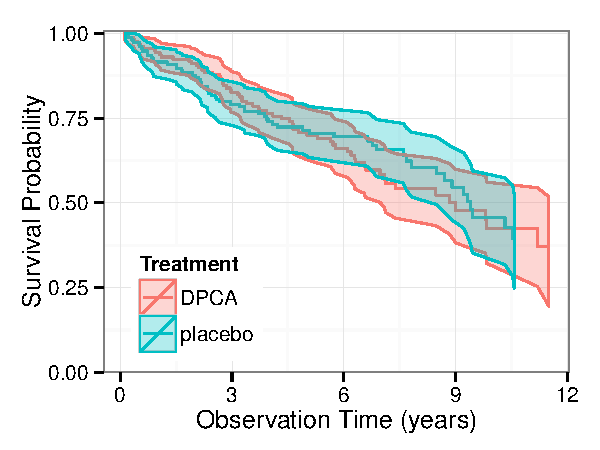
\includegraphics[width=\maxwidth]{figure/rfs-plot_gg_survival-1} 

}

\caption[Kaplan--Meier pbc data survival estimates comparing the treatment with placebo]{Kaplan--Meier pbc data survival estimates comparing the treatment with placebo. Mean survival with shaded 95\% condfidence band.\label{fig:plot_gg_survival}}
\end{figure}
\end{Schunk}

In Chapter 4,~\cite{fleming:1991} use partial likelihood methods to build a linear model with log transformations on some variables. The final, biologically reasonable model is detailed in Table~\ref{T:FHmodel} for later comparison with our random forest model results.

% latex table generated in R 3.1.2 by xtable 1.7-4 package
% Sun Jan  4 09:53:42 2015
\begin{table}[ht]
\centering
{\footnotesize
\begin{tabular}{rrrr}
  \toprule
 & Coef. & Std. Err. & Z stat. \\ 
  \midrule
Age & 0.0333 & 0.0087 & 3.8400 \\ 
   \rowcolor[gray]{0.95}log(Albumin) & -3.0553 & 0.7241 & -4.2200 \\ 
  log(Bilirubin) & 0.8792 & 0.0987 & 8.9000 \\ 
   \rowcolor[gray]{0.95}Edema & 0.7847 & 0.2991 & 2.6200 \\ 
  log(Prothrombin Time) & 3.0157 & 1.0238 & 2.9500 \\ 
   \rowcolor[gray]{0.95} \bottomrule
\end{tabular}
}
\caption{Regression model with log transformations of continuous variables, 312 randomized cases with PBC.} 
\label{T:FHmodel}
\end{table}


In Figure~\ref{fig:plot_gg_survival}, we demonstrated grouping on a categorical variable (\code{treatment}). However, with the exception of \code{edema}, all variables in the~\cite{fleming:1991} model are continuous. To demonstrate plotting grouped survival on a continuous variable, we examine KM estimates of survival by stratified bilirubin grouping from~\cite{fleming:1991} Figure 4.4.2. 

The following code block duplicates the \code{pbc.trial} data for this exercise. We set up the \code{bili} groups using the \code{cut} function with intervals matching the reference figure. For this example we combine the data generation and plot steps into a single line of code. The \code{error} argument of the \code{plot.gg_survival} is used to control display of the confidence bands. We suppress the intervals for this figure with \code{error = "none"} and again modify the plot display with \pkg{ggplot2} commands as before to generate Figure~\ref{fig:gg_survival-bili}.

\begin{Schunk}
\begin{Sinput}
R> # Duplicate the trial data
R> pbc.bili <- pbc.trial
R> 
R> # Group by bilirubin values 
R> pbc.bili$bili_grp <- cut(pbc.trial$bili, 
+                          breaks = c(0, .8, 1.3, 3.4, 
+                                   max(pbc.trial$bili)))
R> 
R> # plot the gg_survival object directly
R> plot(gg_survival(interval = "years",censor = "status", 
+                  strat= "bili_grp", data = pbc.bili),
+      error = "none") +
+   labs(y = "Survival Probability", 
+        x = "Observation Time (years)", 
+        color = "Bilirubin")
\end{Sinput}
\begin{figure}[!htpb]

{\centering 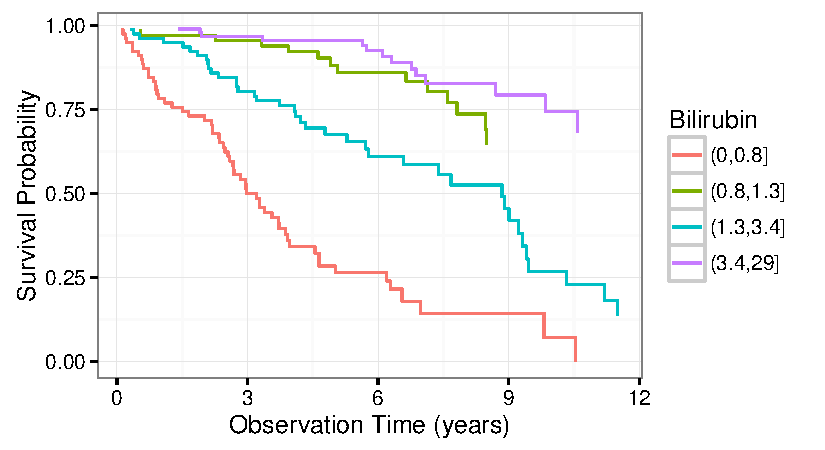
\includegraphics[width=\maxwidth]{figure/rfs-gg_survival-bili-1} 

}

\caption{Kaplan--Meier pbc data survival estimates comparing Bilirubin measures. Groups defined in~\cite{fleming:1991}.\label{fig:gg_survival-bili}}
\end{figure}
\end{Schunk}


\section{Random Survival Forest}\label{S:rfsrcGrow}
A Random Forest~\citep{Breiman:2001} is grown by \emph{bagging}~\citep{Breiman:1996} a collection of \emph{classification and regression trees} (CART)~\citep{cart:1984}. The method uses a set of $B$ \emph{bootstrap}~\citep{bootstrap:1994} samples, growing an independent tree model on each sub-sample of the population. Each tree is grown by recursively partitioning the population based on optimization of a \emph{split rule} over the $p$-dimensional covariate space. At each split, a subset of $m \le p$ candidate variables are tested for the split rule optimization, dividing each node into two daughter nodes. Each daughter node is then split again until the process reaches the \emph{stopping criteria} of either \emph{node purity} or \emph{node member size}, which defines the set of \emph{terminal (unsplit) nodes} for the tree. In regression trees, node impurity is measured by mean squared error, whereas in classification problems, the Gini index is used~\citep{Friedman:2000} . 

Random Forests sort each training set observation into one unique terminal node per tree. Tree estimates for each observation are constructed at each terminal node, among the terminal node members. The Random Forest estimate for each observation is then calculated by aggregating, averaging (regression) or votes (classification), the terminal node results across the collection of $B$ trees.

Random Forests for survival~\citep{Ishwaran:2007, Ishwaran:2008} (RF-S) are an extension of~\cite{Breiman:2001} Random Forests for right censored time to event data. A forest of survival trees is grown using a log-rank splitting rule to select the optimal candidate variables. Survival estimate for each observation are constructed with a Kaplan--Meier (KM) estimator within each terminal node, at each event time. 

Random Forests for survival adaptively discover nonlinear effects and interactions and are fully nonparametric. Averaging over trees, with randomization while growing a tree, enables RF-S to approximate complex survival functions, including non-proportional hazards, while maintaining low prediction error. \cite{Ishwaran:2010a} showed that RF-S is uniformly consistent and that survival forests have a uniform approximating property in finite-sample settings, a property not possessed by individual survival trees.

The \pkg{randomForestSRC} \code{rfsrc} function call grows the forest, determining the type of forest by the response supplied in the \code{formula} argument. In the following code block, we grow a random forest for survival, by passing a survival (\code{Surv}) object to the forest. The forest uses all remaining variables in the \code{pbc.trial} data set to generate survival estimates. 

\begin{Schunk}
\begin{Sinput}
R> # Grow and store the random survival forest
R> # Use random splitting (nsplit = 10) and impute 
R> # missing values (na.action = "na.impute")
R> rfsrc_pbc <- rfsrc(Surv(years, status) ~ ., 
+                    data = pbc.trial, 
+                    nsplit = 10, 
+                    na.action = "na.impute")
R> 
R> # Print the forest summary
R> rfsrc_pbc
\end{Sinput}
\end{Schunk}

\begin{Schunk}
\begin{Soutput}
                         Sample size: 312
                    Number of deaths: 125
                    Was data imputed: yes
                     Number of trees: 1000
          Minimum terminal node size: 3
       Average no. of terminal nodes: 60.071
No. of variables tried at each split: 5
              Total no. of variables: 17
                            Analysis: RSF
                              Family: surv
                      Splitting rule: logrank *random*
       Number of random split points: 10
                          Error rate: 15.99%
\end{Soutput}
\end{Schunk}

The \code{print.rfsrc} function returns information on how the random forest was grown. Here the \code{family = "surv"} forest has \code{ntree = 1000} trees (the default \code{ntree} argument). We used \code{nsplit = 10} random split points to select random split rule, instead of an optimization on each variable at each split for performance reasons. 

\subsection{Generalization error}

One advantage of Random Forests is a built in generalization error estimate. Each bootstrap sample selects approximately $63.2\%$ of the population on average. The remaining $36.8\%$ of observations, the Out-of-Bag~\citep{BreimanOOB:1996e} (OOB) sample, can be used as a hold out test set for each tree. An OOB prediction error estimate can be calculated for each observation by predicting the response over the set of trees which were NOT trained with that particular observation. Out-of-Bag prediction error estimates have been shown to be nearly identical to $n$--fold cross validation estimates~\citep{StatisticalLearning:2009}. This feature of Random Forests allows us to obtain both model fit and validation in one pass of the algorithm.


The \code{gg_error} function operates on the random forest object to extract the error estimates from the forest is grown. The following code block first creates a \code{gg_error} object, then uses the \code{plot.gg_error} function to create a \pkg{ggplot2} object for display.

\begin{Schunk}
\begin{figure}[!htpb]

{\centering 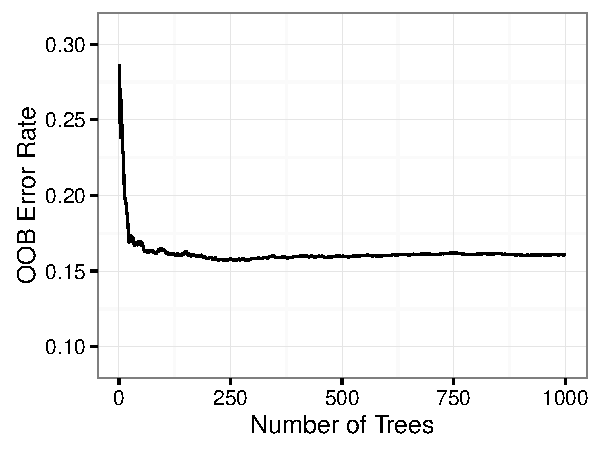
\includegraphics[width=\maxwidth]{figure/rfs-errorPlot-1} 

}

\caption[Random forest prediction error estimates as a function of the number of trees in the forest]{Random forest prediction error estimates as a function of the number of trees in the forest.\label{fig:errorPlot}}
\end{figure}
\end{Schunk}

This figure demonstrates that it does not take a large number of trees to stabilize the forest prediction error estimate. However, to ensure that each variable has enough of a chance to be included in the forest prediction process, we do want to create a rather large random forest of trees. 

\subsection{Training Set Prediction}\label{S:prediction}

The \code{gg_rfsrc} function extracts the OOB prediction estimates from the random forest. This code block executes the the data extraction and plotting in one line, since we are not interested in holding the prediction estimates for later reuse. Also note that we again add in the additional \pkg{ggplot2} commands to modify the display of the plot object. Each of the `ggRandomForests` S3 plot commands return \pkg{ggplot2} objects, which we can also store for modification or reuse later in the analysis. 

\begin{Schunk}
\begin{figure}[!htpb]

{\centering 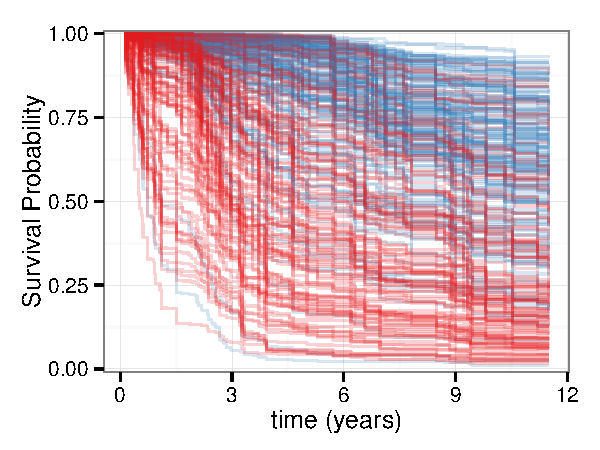
\includegraphics[width=\maxwidth]{figure/rfs-rfsrc-plot-1} 

}

\caption[Random forest predicted survival]{Random forest predicted survival. Blue lines correspond to censored observations, red lines correspond to patients who experienced the event (death).\label{fig:rfsrc-plot}}
\end{figure}
\end{Schunk}


Figure~\ref{fig:rfsrc-plot} shows the predicted survival from an RF-S model, where censored device prediction is colored in blue, and devices experiencing an event are colored in red. 

\begin{Schunk}
\begin{figure}[!htpb]

{\centering 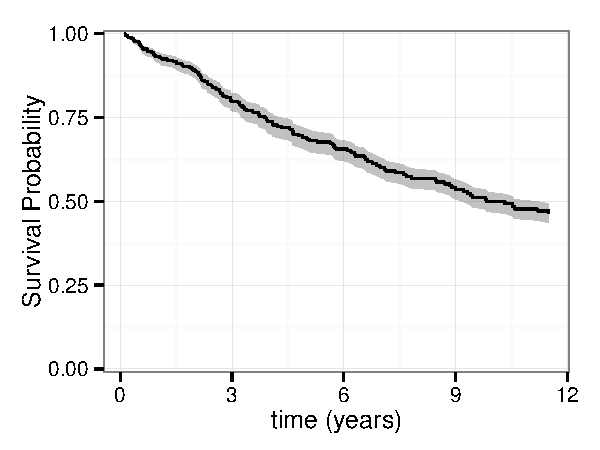
\includegraphics[width=\maxwidth]{figure/rfs-rfsrc-mean-1} 

}

\caption[Mean value random forest predicted survival with shaded 95\% confidence band]{Mean value random forest predicted survival with shaded 95\% confidence band.\label{fig:rfsrc-mean}}
\end{figure}
\end{Schunk}

\begin{Schunk}
\begin{figure}[!htpb]

{\centering 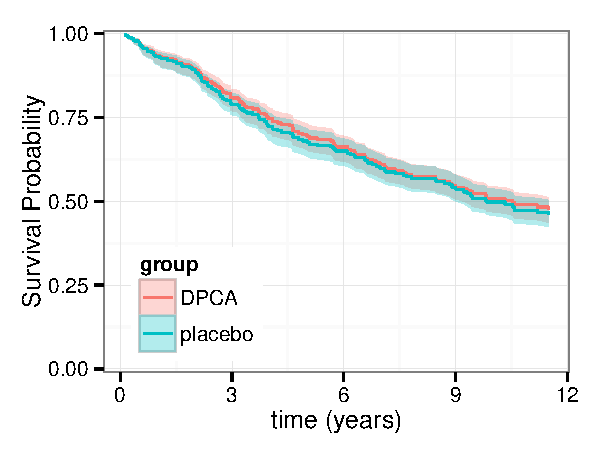
\includegraphics[width=\maxwidth]{figure/rfs-rfsrc-mean2-1} 

}

\caption[Mean value random forest predicted survival with shaded 95\% confidence band]{Mean value random forest predicted survival with shaded 95\% confidence band. Treatment effects (TODO!!!)\label{fig:rfsrc-mean2}}
\end{figure}
\end{Schunk}

\subsection{Imputation}\label{S:imputation}

There are two modeling issues when dealing with missing data values: How does the algorithm build a model when values are missing from the training data, and how does the algorithm predict a response when values are missing from the test data. The standard procedure for linear models is to either remove or impute the missing data values. Removing the missingness is done by either removing the variable with missing values (column wise) or removing the observations (row wise) impute missing values before fitting a model. Removal is a simple solution, but may bias results when observations or variables are scarce. 

The \pkg{randomForestSRC} package has an internal missing value imputation algorithm with in the \code{rfsrc} function~\cite{Ishwaran:2008}. Rather than impute all missing values before growing the forest, the algorithm takes a ``just in time'' approach. At each node split, the set of $m$ candidate variables is checked for missing data. Missing values are imputed by randomly drawing values from non-missing values within the node before calculating the split-statistic on observations without missing data. The imputed values are used to sort observations into the subsequent daughter nodes and then discarded before the next split occurs. The process is repeated until terminal nodes are reached. 

A final imputation step can be used to fill in missing values from within the terminal nodes. This step uses a process to the previous imputation but uses the OOB non-missing terminal node data for the random draws. These values are aggregated (averaging for continuous variables, voting for categorical variables) over the $B$ trees in the forest to estimate an imputed data set. By default, the missing values are not filled into the training data, but are available within the forest object.

At each imputaton step, the random forest assumes that similar observations are grouped together within each node. The random draws to fill in missing data do not bias the split rule, but only sort observations similar in non-missing data into like nodes. A feature if this approach is the ability of predicting on test set observations without having to impute missing values. 

\subsection{Test Set Predictions}

\begin{Schunk}
\begin{Sinput}
R> # Predict survival for 106 patients not in randomized trial
R> rfsrc_pbc_test <- predict(rfsrc_pbc, 
+                     newdata = pbc.test,
+                     na.action = "na.impute")
R> 
R> # Print prediction summary  
R> rfsrc_pbc_test
\end{Sinput}
\end{Schunk}
\begin{Schunk}
\begin{Soutput}
  Sample size of test (predict) data: 106
       Number of deaths in test data: 36
               Was test data imputed: yes
                Number of grow trees: 1000
  Average no. of grow terminal nodes: 59.902
         Total no. of grow variables: 17
                            Analysis: RSF
                              Family: surv
                 Test set error rate: 19.1%
\end{Soutput}
\end{Schunk}

\begin{Schunk}
\begin{figure}[!htpb]

{\centering 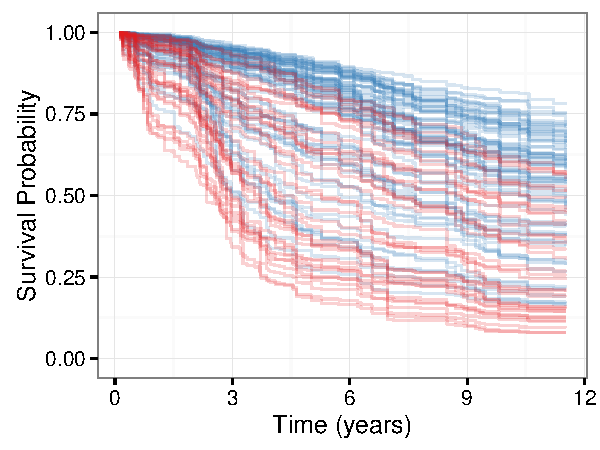
\includegraphics[width=\maxwidth]{figure/rfs-predictPlot-1} 

}

\caption[Test set prediction]{Test set prediction: 106 observations.\label{fig:predictPlot}}
\end{figure}
\end{Schunk}

\section{Variable Selection}\label{S:variableselection}

Random forests are not parsimonious, but use all variables available in the construction of a response predictor. Also, unlike parametric models, Random Forests do not require the explicit specification of the functional form of covariates to the response. Therefore there is no explicit p-value/significance test for variable selection with a random forest model. Instead, RF ascertain which variables contribute to the prediction through the split rule optimization, optimally choosing variables which separate observations. We use two separate approaches to explore the RF selection process, Variable Importance (Section~\ref{S:vimp}) and Minimal Depth (Section~\ref{S:minimalDepth}).

\subsection{Variable Importance}\label{S:vimp}

\emph{Variable importance} (VIMP) was originally defined in CART using a measure involving surrogate variables (see Chapter 5 of~\cite{cart:1984}). The most popular VIMP method uses a prediction error approach involving "noising-up" each variable in turn. VIMP for a variable $x_v$ is the difference between prediction error when $x_v$ is noised up by randomly permuting its values, compared to prediction error under the observed values~\citep{Breiman:2001,Liaw:2002,Ishwaran:2007,Ishwaran:2008}.

Since VIMP is the difference between OOB prediction error before and after permutation, a large VIMP value indicates that misspecification detracts from the variable predictive accuracy in the forest. VIMP close to zero indicates the variable contributes nothing to predictive accuracy, and negative values indicate the predictive accuracy \emph{improves} when the variable is mispecified. In the later case, we assume noise is more informative than the true variable. As such, we ignore variables with negative and near zero values of VIMP, relying on large positive values to indicate that the predictive power of the forest is dependent on those variables. 

The \code{gg_vimp} function extracts VIMP measures for each of the variables used to grow the forest. The \code{plot.gg_vimp} function shows the variables, in VIMP rank order. Figure~\ref{fig:rf-vimp} details VIMP ranking for the \code{pbc} trial, from the largest (serum bilirubin) at the top, to smallest (Treatment) at the bottom. VIMP measures are shown using bars to compare the scale of the error increase under permutation and colored by the sign of the measure (red for negative values). 

\begin{Schunk}
\begin{Sinput}
R> plot.gg_vimp(rfsrc_pbc, lbls = st.labs) + 
+   theme(legend.position = c(.8,.2))+
+   labs(fill = "VIMP > 0")+
+   scale_fill_brewer(palette = "Set1")
\end{Sinput}
\begin{figure}[!htpb]

{\centering 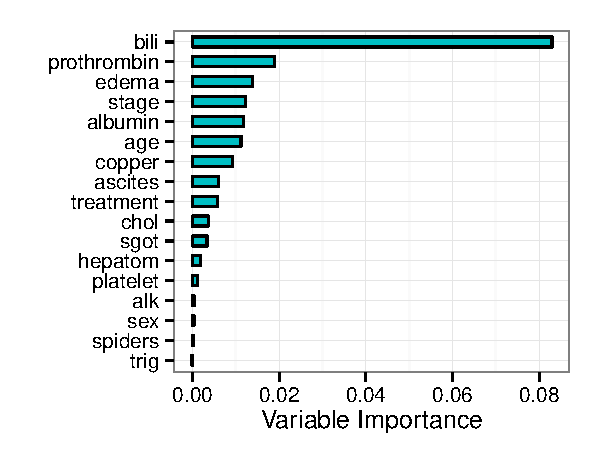
\includegraphics[width=\maxwidth]{figure/rfs-rf-vimp-1} 

}

\caption[Random forest variable Importance (VIMP)]{Random forest variable Importance (VIMP). Blue bars indicate important variables (positive VIMP), red indicates noise variables (negative VIMP).\label{fig:rf-vimp}}
\end{figure}
\end{Schunk}

Note that four of the five highest ranking variables by VIMP match those selected by the~\cite{fleming:1991} model listed in Table~\ref{T:FHmodel}, with urine copper (2) ranking higher than age (8).  

\subsection{Minimal Depth}\label{S:minimalDepth}

In VIMP, prognostic risk factors are determined by testing the forest prediction under alternative data settings, ranking the most important variables according to their impact on predictive ability of the forest. An alternative method uses inspection of the forest construction to rank variables. \emph{Minimal depth}~\citep{Ishwaran:2010, Ishwaran:2011} assumes that variables with high impact on the prediction are those that most frequently split nodes nearest to the trunks of the trees (i.e. at the root node) where they partition large samples of the population. 

Within a tree, node levels are numbered based on their relative distance to the trunk of the tree (with the root at 0). Minimal depth measures the important risk factors by averaging the depth of the first split for each variable over all trees within the forest. Lower values of this measure indicate variables important in splitting large groups of patients. 

The \emph{maximal subtree} for a variable $x$ is the largest subtree whose root node splits on $x$. All parent nodes of $x$'s maximal subtree have nodes that split on variables other than $x$. The largest maximal subtree possible is at the root node. If a variable does not split the root node, it can have more than one maximal subtree, or a maximal subtree may also not exist if there are no splits on the variable. The minimal depth of a variables is a surrogate measure of predictiveness of the variable. The smaller the minimal depth, the more impact the variable has sorting observations, and therefore on the forest prediction. 

The \pkg{randomForestSRC} \code{var.select} function uses the minimal depth methodology for variable selection, returning an object with both minimal depth and vimp measures. The \pkg{ggRandomForests} \code{gg_minimal_depth} function is analogous to the \code{gg_vimp} function for minimal depth. Variables are ranked from most important at the top (minimal depth measure), to least at the bottom (maximal minimal depth). The vertical dashed line indicates the minimal depth threshold where smaller minimal depth values indicate higher importance and larger indicate lower importance.

\begin{Schunk}
\begin{Sinput}
R> varsel_pbc <- var.select(rfsrc_pbc)
R> ggMindepth <- gg_minimal_depth(varsel_pbc, lbls = st.labs)
R> print(ggMindepth)
\end{Sinput}
\end{Schunk}

\begin{Schunk}
\begin{Soutput}
-----------------------------------------------------------
gg_minimal_depth
model size         : 12 
depth threshold    : 5.5905 

PE :[1] 15.994
-----------------------------------------------------------

Top variables:
            depth  vimp
bili        1.686 0.069
albumin     2.559 0.014
copper      2.684 0.018
prothrombin 2.986 0.011
chol        3.274 0.005
edema       3.365 0.017
age         3.489 0.009
platelet    3.681 0.002
sgot        3.778 0.007
alk         3.913 0.001
trig        4.418 0.000
stage       4.655 0.008
-----------------------------------------------------------
\end{Soutput}
\end{Schunk}


In general, the selection of variables according to VIMP is to examine the values, looking for some point along the ranking where there is a large difference in VIMP measures. The minimal depth threshold method has a more quantitative approach to determine a selection threshold. Given minimal depth is a quantitative property of the forest construction, \cite{Ishwaran:2010} also derive an analytic threshold for evidence of variable impact. A simple optimistic threshold rule uses the mean of the minimal depth distribution, classifying variables with minimal depth lower than this threshold as important in forest prediction. The minimal depth plot for our model indicates there are twelve variables which have a higher impact (minimal depth below the mean value threshold) than the remaining five. 

\begin{Schunk}
\begin{Sinput}
R> plot(ggMindepth, lbls = st.labs)
\end{Sinput}
\begin{figure}[!htpb]

{\centering 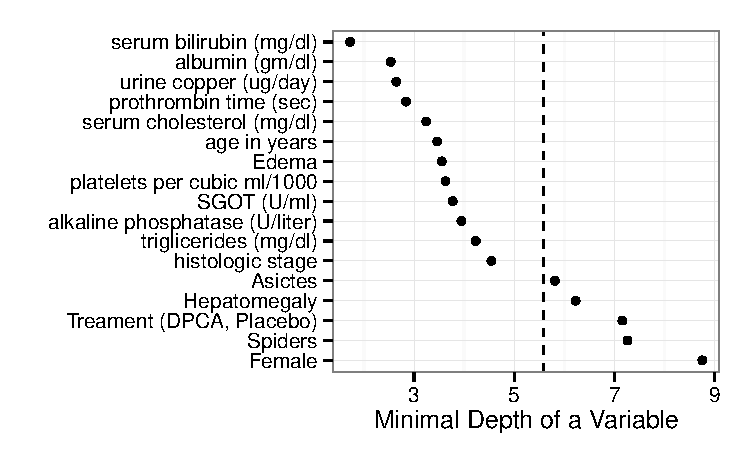
\includegraphics[width=\maxwidth]{figure/rfs-mindepth-plot-1} 

}

\caption[Minimal Depth variable selection]{Minimal Depth variable selection. Low minimal depth indicates important variables. The dashed line is the threshold of maximum value for variable selection.\label{fig:mindepth-plot}}
\end{figure}
\end{Schunk}


The minimal depth plot of Figure~\ref{fig:mindepth-plot} is similar to the VIMP plot in Figure~\ref{fig:rf-vimp}, ranking variables from most important at the top (minimal depth measure), to least at the bottom (maximal minimal depth). The vertical dashed line indicates the minimal depth threshold where smaller minimal depth values indicate higher importance and larger indicate lower importance.

Since the VIMP and Minimal Depth measures use different criteria, we expect the variable ranking to be somewhat different. We use \code{gg_minimal_vimp} function to compare rankings between minimal depth and VIMP.

\begin{Schunk}
\begin{figure}[!htpb]

{\centering 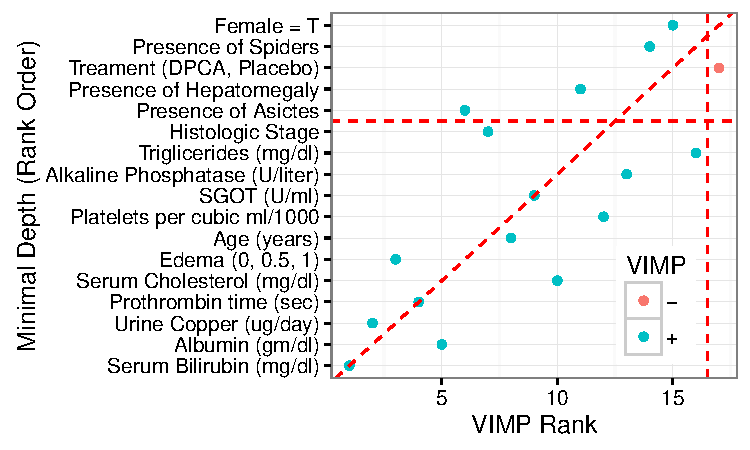
\includegraphics[width=\maxwidth]{figure/rfs-depthVimp-1} 

}

\caption[Comparing Minimal Depth and Vimp rankings]{Comparing Minimal Depth and Vimp rankings. Points on the red dashed line are ranked equivalently, points below have higher VIMP, those above have higher minimal depth ranking. Variables are colored by the sign of the VIMP measure.\label{fig:depthVimp}}
\end{figure}
\end{Schunk}

The points along the red dashed line indicates where the measures are in agreement. Points above the red dashed line are ranked higher by VIMP than by minimal depth, indicating the variables are sensitive to misspecification. Those below the line have a higher minimal depth ranking, indicating they are better at dividing large portions of the population. The further the points are from the line, the more the discrepancy between measures. The construction of this figure is skewed towards a minimal depth approach, by ranking variables along the y-axis, though points are colored by the sign of VIMP. 

In our example, both minimal depth and VIMP indicate the strong relation of serum bilirubin to the forest prediction, and agrees reasonably well with the~\cite{fleming:1991} model. We now turn to investigating how these, and other variables, are related to the predicted response.

\section{Variable Dependence}\label{S:dependence}

As random forests are not a parsimonious methodology, we use the minimal depth and VIMP measures to reduce the number of variables we need to examine to a manageable subset. Once we have an idea of which variables contribute most to the predictive accuracy of the forest, we would like to know how the response depends on these variables.

Although often characterized as a \emph{black box} method, it is possible to express a random forest in functional form. In the end the forest predictor is some function, although complex, of the predictor variables $\hat{f}_{rf} = f(x).$ We use graphical methods to examine the forest predicted response dependency on covariates. We again have two options, variable dependence (Section~\ref{S:variabledependence}) plots are quick and easy to generate, and partial dependence(Section~\ref{S:partialdependence}) plots are computationally intensive but give us a risk adjusted look at variable dependence. 

\subsection{Marginal Dependence}\label{S:variabledependence}

\emph{Variable dependence} plots show the predicted response as a function of a covariate of interest, where each observation is represented by a point on the plot. Each predicted point represents an individual observation, dependent on the full combination of all other covariates, not only on the covariate of interest. Interpretation of variable dependence plots can only be in general terms, as point predictions are a function of all covariates in that particular observation. However, variable dependence is straight forward to calculate, involving only the getting the predicted response for each observation.

In survival settings, we must also account for the additional dimension of time. In this case, we plot the response at a specific time point of interest, for example survival at 1 or 3 years, as shown by the vertical dashed line in Figure~\ref{fig:rfsrc-plot3Mnth}. The point prediction is then the predicted value of each curve at that intersecting time line, and plot that against the covariate value for that observations
\begin{Schunk}
\begin{Sinput}
R> ggRFsrc + 
+   geom_vline(aes(xintercept = c(1, 3)), linetype = "dashed") + 
+   coord_cartesian(x = c(0, 4))
\end{Sinput}
\begin{figure}[!htpb]

{\centering 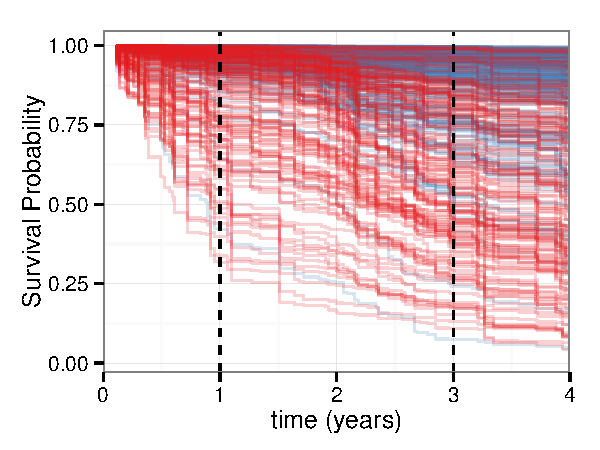
\includegraphics[width=\maxwidth]{figure/rfs-rfsrc-plot3Mnth-1} 

}

\caption[Random forest OOB predicted patient survival]{Random forest OOB predicted patient survival. Red curves correspond to patients which have died, blue corresponds to alive (or censored) cases. Vertical dashed lines indicate the 1 and 3 year survival estimates.\label{fig:rfsrc-plot3Mnth}}
\end{figure}
\end{Schunk}

, shown in Figure~\ref{fig:variable-plot}. Again censored cases are shown in blue circles, events are indicated by the red "x" symbols. Each predicted point is dependent on the full combination of all other covariates, not only on the covariate displayed in the dependence plot, so interpretation of these variable dependence plots can only be in general terms. The smooth loess line~\citep{cleveland:1981, cleveland:1988} indicates the trend of the prediction over surgical date progression.


\begin{Schunk}
\begin{Sinput}
R> # Get the minimal depth selected variables
R> xvar <- varsel_pbc$topvars
R> 
R> # Data generation
R> ggrf <- gg_variable(rfsrc_pbc, time = c(1, 3), 
+                     time.labels = c("1 Year", "3 Years"))
R> 
R> # Plot the bilirubin variable dependence plot
R> plot(ggrf, xvar = "bili", se = .95, alpha = .3) + 
+   labs(y = "Survival", x = st.labs["bili"]) + 
+   theme(legend.position = "none") + 
+   scale_color_manual(values = strCol, labels = event.labels) + 
+   scale_shape_manual(values = event.marks, labels = event.labels)+
+   coord_cartesian(y = c(-.01,1.01))
\end{Sinput}
\begin{figure}[!htpb]

{\centering 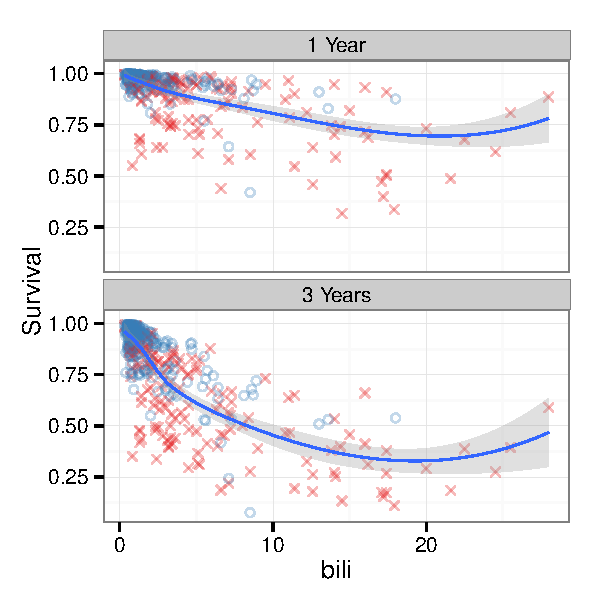
\includegraphics[width=\maxwidth]{figure/rfs-variable-plotbili-1} 

}

\caption[Bilirubin variable dependence at 1 and 3 years]{Bilirubin variable dependence at 1 and 3 years. Individual cases are marked with blue circles (alive or censored) and red xs (dead). Loess smooth curve with shaded 95\% confidence band indicates the survival trend with increasing bilirubin.\label{fig:variable-plotbili}}
\end{figure}
\end{Schunk}


We use the \code{gg_variable} function call to extract the training set variables and the predicted OOB response from \code{randomForestSRC::rfsrc} and \code{randomForestSRC::predict} objects. In the following code block, we will store the \code{gg_variable} data object for later use, as all remaining variable dependence plots can be constructed from this (\code{gg_v}) object. We will also use the minimal depth selected variables (minimal depth lower than the threshold value) from the previously stored \code{gg_minimal_depth} object (\code{gg_md$topvars}) to filter the variables of interest.

The \code{plot.gg_variable} function call operates in the \code{gg_variable} object. We pass it the list of variables of interest (\code{xvar}) and request a single panel (\code{panel = TRUE}) to display the figures. By default, the \code{plot.gg_variable} function returns a list of \pkg{ggplot2} objects, one figure for each variable named in \code{xvar} argument. The next three arguments are passed to internal \pkg{ggplot2} plotting routines. The \code{se} and \code{span} arguments are used to modify the internal call to \code{geom_smooth} for fitting smooth lines to the data. The \code{alpha} argument lightens the coloring points in the \code{geom_point} call, making it easier to see point over plotting. We also demonstrate modification of the plot labels using the \code{labs} function.


\begin{Schunk}
\begin{Sinput}
R> # Pull the categorical variables
R> xvar.cat <- c("edema", "stage")
R> xvar <- xvar[-which(xvar %in% xvar.cat)]
R> 
R> # plot the next 5 continuous variable dependence plots.
R> plot(ggrf, xvar = xvar[2:6], panel = TRUE, 
+      se = FALSE, alpha = .3, 
+      method = "glm", formula = y~poly(x,2)) + 
+   labs(y = "Survival") + 
+   theme(legend.position = "none") + 
+   scale_color_manual(values = strCol, labels = event.labels) + 
+   scale_shape_manual(values = event.marks, labels = event.labels)+
+   coord_cartesian(y = c(-.01,1.01))
\end{Sinput}
\begin{figure}[!htpb]

{\centering 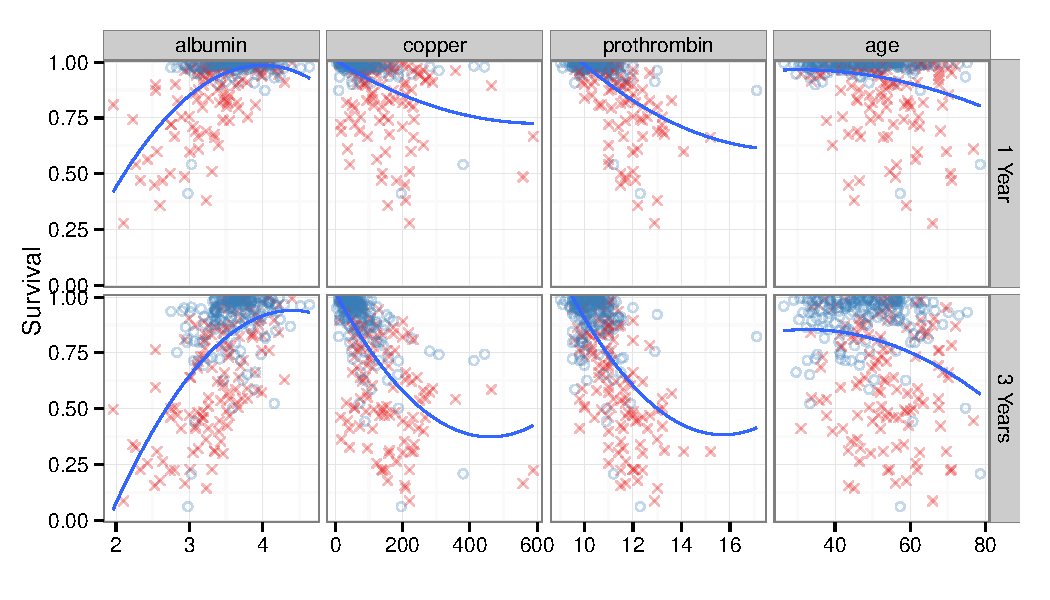
\includegraphics[width=\maxwidth]{figure/rfs-variable-plot-1} 

}

\caption[Bilirubin variable dependence at 1 and 3 years]{Bilirubin variable dependence at 1 and 3 years. Individual cases are marked with blue circles (alive or censored) and red xs (dead). Loess smooth curve with shaded 95\% confidence band indicates the survival trend with increasing bilirubin.\label{fig:variable-plot}}
\end{figure}
\end{Schunk}

The panels are sorted to match the order of variables in the \code{xvar} argument and include a smooth loess line~\citep{cleveland:1981,cleveland:1988} to indicate the trend of the prediction dependence over the covariate values.

There is not a convenient method to panel scatter plots and boxplots together, so we recommend creating panel plots for each variable type separately. Variable dependence plots for categorical variables are constructed using boxplots to show the distribution of the predictions within each category. 

\begin{Schunk}
\begin{Sinput}
R> plot(ggrf, xvar = xvar.cat, panel = TRUE, notch = TRUE, alpha = .3) + 
+   labs(y = "Survival") + 
+   theme(legend.position = "none") + 
+   scale_color_manual(values = strCol, labels = event.labels) + 
+   scale_shape_manual(values = event.marks, labels = event.labels)+
+   coord_cartesian(y = c(-.01,1.02))
\end{Sinput}
\begin{figure}[!htpb]

{\centering 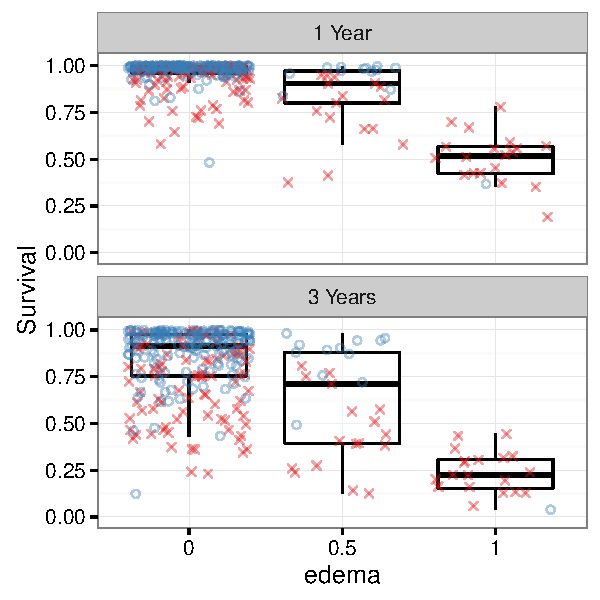
\includegraphics[width=\maxwidth]{figure/rfs-variable-plotCat-1} 

}

\caption[Variable dependence plots at 1 and 3 years for continuous variables age, albumin, copper and prothrombin]{Variable dependence plots at 1 and 3 years for continuous variables age, albumin, copper and prothrombin. Individual cases are marked with blue circles (alive or censored) and red xs (dead). Loess smooth curve indicates the survival trend with increasing variable value.\label{fig:variable-plotCat}}
\end{figure}
\end{Schunk}

\subsection{Partial Dependence}\label{S:partialdependence}

\emph{Partial dependence plots} are a risk adjusted alternative to marginal variable dependence. Partial plots are generated by integrating out the effects of variables beside the covariate of interest. The figures are constructed by selecting points evenly spaced along the distribution of the $X$ variable. For each of these values ($X = x$), we calculate the average Random Forest prediction over all other covariates in $X$ by
\begin{equation}
\tilde{f}(x) = \frac{1}{n} \sum_{i = 1}^n \hat{f}(x, x_{i, o}), 
\label{E:partial}
\end{equation}
where $\hat{f}$ is the predicted response from the random forest and $x_{i, o}$ is the value for all other covariates other than $X = x$ for the observation $i$~\citep{Friedman:2000}. Partial dependence plots in time to event settings are shown at specific time points, similar to variable dependence.

Partial plots are computationally intensive to create, especially when there are a large number of observations. The default parameters for the \code{randomForestSRC::plot.variable} function generate partial dependence estimates at \code{npts = 25} points along the variable of interest. For each point of interest, the \code{plot.variable} function averages \code{n} response predictions. This is repeated for each of the variables of interest and the results are returned for later analysis. 

\begin{Schunk}
\begin{Sinput}
R> # Calculate the 1, 3 and 5 year partial dependence
R> partial_pbc <- lapply(c(1,3,5), function(tm){
+   plot.variable(rfsrc_pbc, surv.type = "surv", 
+                 time = tm, 
+                 xvar.names = xvar, partial = TRUE, 
+                 show.plots = FALSE)
+   })
\end{Sinput}
\end{Schunk}




\begin{Schunk}
\begin{Sinput}
R> # Convert all partial plots to gg_partial objects
R> gg_dta <- lapply(partial_pbc, gg_partial)
R> 
R> # Combine the objects to get multiple time curves 
R> # along variables on a single figure.
R> pbc_ggpart <- combine.gg_partial(gg_dta[[1]], gg_dta[[2]], 
+                                  lbls = c("1 Year", "3 Years"))
R> 
R> 
R> plot(pbc_ggpart[["bili"]], se = FALSE) + 
+   theme(legend.position = c(.2, .2)) + 
+   labs(y = "Survival", 
+        x = st.labs["bili"],
+        color = "Time", shape = "Time")+
+   scale_color_brewer(palette = "Set2")+
+   coord_cartesian(y = c(25,101))
\end{Sinput}
\begin{figure}[!htpb]

{\centering 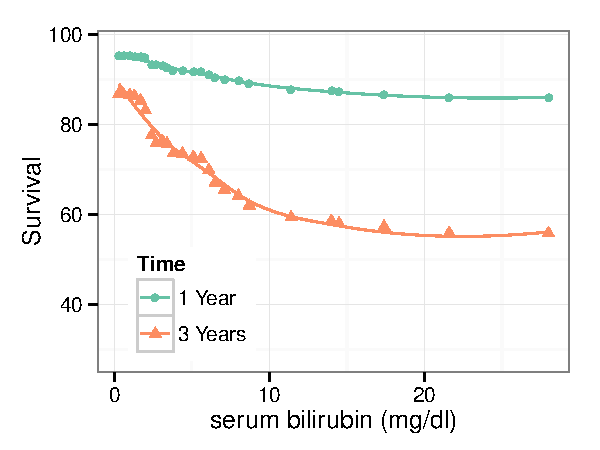
\includegraphics[width=\maxwidth]{figure/rfs-pbc-partial-bili-1} 

}

\caption[Partial dependence plot of (risk adjusted) predicted survival probability as a function of serum bilirubin at 1 year (red circle) and 3 years (blue triangle)]{Partial dependence plot of (risk adjusted) predicted survival probability as a function of serum bilirubin at 1 year (red circle) and 3 years (blue triangle). Loess smooth curves indicates the trend.\label{fig:pbc-partial-bili}}
\end{figure}
\end{Schunk}

Figure~\ref{fig:pbc-partial-bili} shows the partial dependence of one (red) and three (blue) survival on bilirubin. Non-proportional hazards are evident in Figure~\ref{fig:pbc-partial-bili}.

\begin{Schunk}
\begin{Sinput}
R> # Create a temporary holder and remove the stage and edema data
R> ggpart <- pbc_ggpart
R> ggpart$edema <- ggpart$stage <- NULL
R> ggpart$bili <- ggpart$sgot <- ggpart$chol <- NULL
R> ggpart$platelet <- ggpart$trig <- ggpart$alk <- NULL
R> 
R> # Panel plot the remainder.
R> plot(ggpart, se = FALSE, panel = TRUE) + 
+   labs(x = "", y = "Survival", color = "Time", shape = "Time") +
+   scale_color_brewer(palette = "Set2") + 
+   theme(legend.position = c(.2, .15)) + 
+   coord_cartesian(y = c(25,101))
\end{Sinput}
\begin{figure}[!htpb]

{\centering 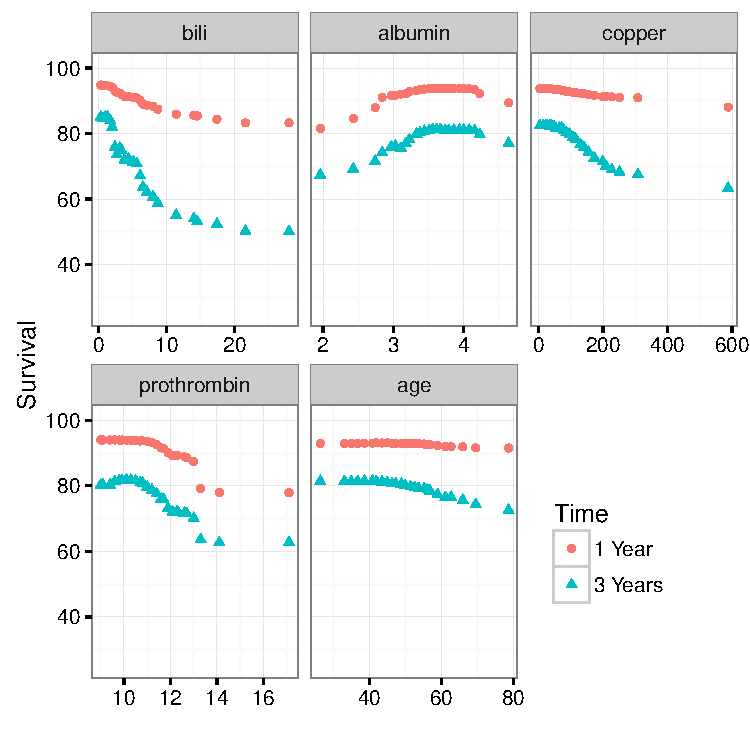
\includegraphics[width=\maxwidth]{figure/rfs-pbc-partial-panel-1} 

}

\caption[Partial dependence plot of (risk adjusted) predicted survival probability as a function continuous variables prothrombin time, albumin, age and urin copper at 1 year (red circle) and 3 years (blue triangle)]{Partial dependence plot of (risk adjusted) predicted survival probability as a function continuous variables prothrombin time, albumin, age and urin copper at 1 year (red circle) and 3 years (blue triangle).\label{fig:pbc-partial-panel}}
\end{figure}
\end{Schunk}

We again order the panels by minimal depth ranking. We see again how the  variables are strongly related to survival, making the partial dependence of the remaining variables look flat. We also see strong nonlinearity of these variables.

\begin{Schunk}
\begin{Sinput}
R> ggpart <- vector("list", length=2)
R> ggpart[[1]] <- pbc_ggpart[["edema"]]
R> ggpart[[2]] <- pbc_ggpart[["stage"]]
R> names(ggpart) <- c("edema", "stage")
R> class(ggpart) <- c("gg_partial_list", class(ggpart))
R> 
R> plot.gg_partial_list(ggpart, panel=TRUE,
+                      notch = TRUE, alpha = .3, outlier.shape = NA) + 
+   labs(x = "", y = "Survival (%)", color="Time", shape="Time")+
+   scale_color_brewer(palette = "Set2")+
+   theme(legend.position = c(.2, .2))+
+   coord_cartesian(y = c(25,101))
\end{Sinput}
\begin{figure}[!htpb]

{\centering 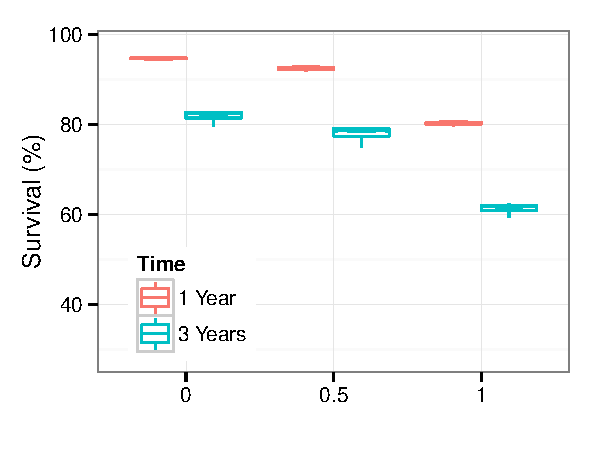
\includegraphics[width=\maxwidth]{figure/rfs-pbc-partial-edema-1} 

}

\caption[Partial dependence plot of (risk adjusted) predicted survival probability as a function of edema (categorical variable) at 1 year (red) and 3 years (blue triangle)]{Partial dependence plot of (risk adjusted) predicted survival probability as a function of edema (categorical variable) at 1 year (red) and 3 years (blue triangle). Points indicate risk adjusted prediction for all patients within each edema group. Box plots indicate distributional properties within each group.\label{fig:pbc-partial-edema}}
\end{figure}
\end{Schunk}

We could stop here, indicating that the RF analysis has found these ten variables to be important in predicting the median home values. That strongest associations to home values where there is a . However, we may also be interested in investigating how variables these work together to help random forest prediction.


\section{Variable Interactions}\label{S:interactions}

Using the different variable dependence measures, it is also possible to calculate measures of pairwise interactions among variables. Recall that minimal depth measure is defined by averaging the tree depth of variable $i$ relative to the root node. To detect interactions, this calculation can be modified to measure the minimal depth of a variable $j$ with respect to the maximal subtree for variable $i$~\citep{Ishwaran:2010,Ishwaran:2011}.

The \code{randomForestSRC::find.interaction} function traverses the forest, calculating all pairwise minimal depth interactions, and returns a $p \times p$ matrix of interaction measures. The diagonal terms are normalized to the root node, and off diagonal terms are normalized measures of pairwise variable interaction. 

\begin{Schunk}
\begin{Sinput}
R> interaction_pbc <- find.interaction(rfsrc_pbc)
R> 
R> ggint <- gg_interaction(interaction_pbc)
\end{Sinput}
\end{Schunk}



The \code{gg_interaction} function wraps the \code{find.interaction} matrix for use with the provided S3 plot and print functions. The \code{xvar} argument indicates which variables we're interested in looking at. We again use the cache strategy, and collect the figures together using the \code{panel = TRUE} option.

\begin{Schunk}
\begin{Sinput}
R> plot(ggint, xvar = xvar) + 
+   labs(y = "Interactive Minimal Depth") + 
+   theme(legend.position = "none")
\end{Sinput}
\begin{figure}[!htpb]

{\centering 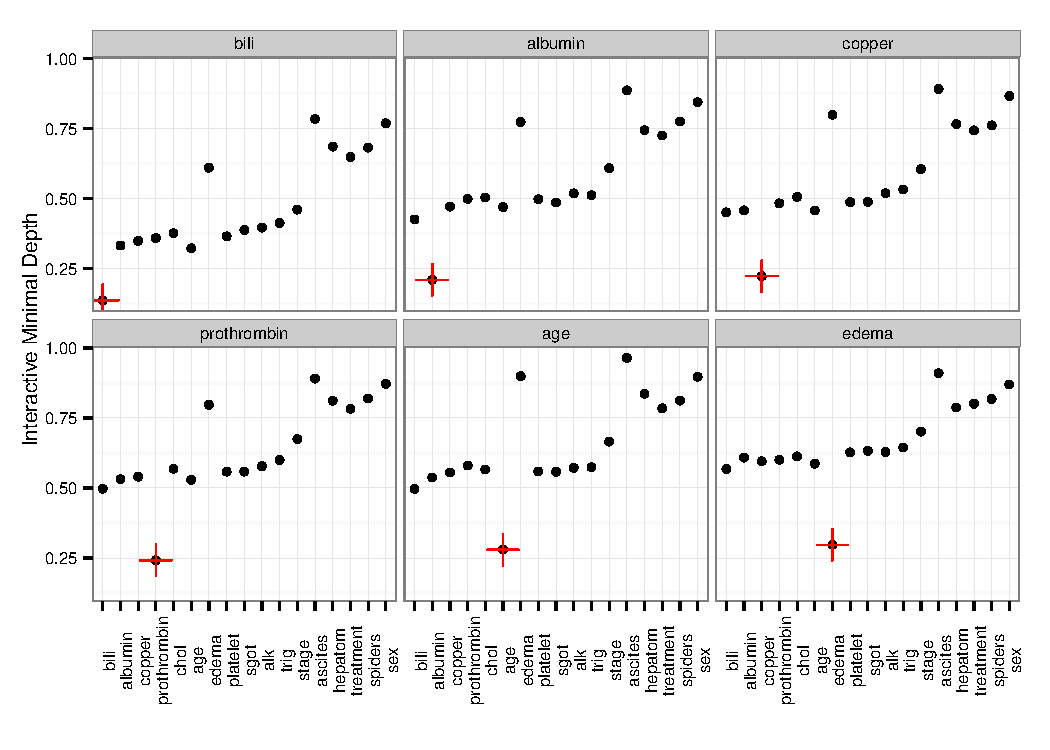
\includegraphics[width=\maxwidth]{figure/rfs-interactionPanel-1} 

}

\caption[Minimal depth variable interaction panel with prothrombin time, albumin, urine copper and edema]{Minimal depth variable interaction panel with prothrombin time, albumin, urine copper and edema. Higher values indicate lower interactivity with target variable.\label{fig:interactionPanel}}
\end{figure}
\end{Schunk}

The \code{gg_interaction} figure plots the interactions for the target variable (shown in the red cross) with interaction scores for all remaining variables. We expect the covariate with lowest minimal depth (`bili`) to be associated with almost all other variables, as it typically splits close to the root node, so viewed alone it may not be as informative as looking at a collection of interactive depth plots. Scanning across the panels, we see each successive target depth increasing, as expected. We also see the interactive variables increasing with increasing target depth. 

\section{Conditional Dependence Plots}\label{S:coplots}

Conditioning plots (coplots)~\citep{chambers:1992,cleveland:1993}  are a powerful visualization tool to efficiently study how a response depends on two or more variables~\citep{cleveland:1993}. The method allows us to view data by grouping observations on some conditional membership. The simplest example involves a categorical variable, where we plot our data conditional on class membership, for instance on the Charles river logical variable. We can view a coplot as a stratified variable dependence plot, indicating trends in the RF prediction results within panels of group membership.

Interactions with categorical data are straight forward, and can be generated directly from variable dependence plots. Recall the 1 year variable dependence for Billirubin, shown in Figure~\ref{fig:var_dep}. 
\begin{Schunk}
\begin{Sinput}
R> ggvar <- gg_variable(rfsrc_pbc, time = 1)
R> ggvar$stage <- paste("stage = ", ggvar$stage, sep = "")
R> 
R> var_dep <- plot(ggvar, xvar = "bili", 
+                 method = "glm",
+                 alpha = .5, se = FALSE) + 
+   labs(y = "Survival", 
+        x = st.labs["bili"]) + 
+   theme(legend.position = "none") + 
+   scale_color_manual(values = strCol, labels = event.labels) + 
+   scale_shape_manual(values = event.marks, labels = event.labels)+
+   coord_cartesian(y = c(-.01,1.01))
R> 
R> show(var_dep)
\end{Sinput}
\begin{figure}[!htpb]

{\centering 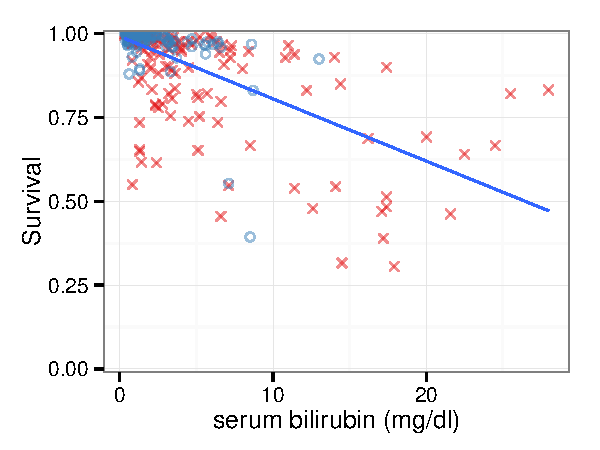
\includegraphics[width=\maxwidth]{figure/rfs-var_dep-1} 

}

\caption[Variable dependence plot]{Variable dependence plot. Survival at 1 year against bilirubin. Individual cases are marked with blue circles (alive or censored) and red x (dead). Loess smooth curve indicates the trend as bilirubin  increases.\label{fig:var_dep}}
\end{figure}
\end{Schunk}

We can view the conditional dependence of survival against bilirubin, versus other categorical covariates, say \code{edema} and \code{stage} (categorical variables), by adding a facet argument.
\begin{Schunk}
\begin{Sinput}
R> var_dep + 
+   facet_grid(edema~stage)
\end{Sinput}
\begin{figure}[!htpb]

{\centering 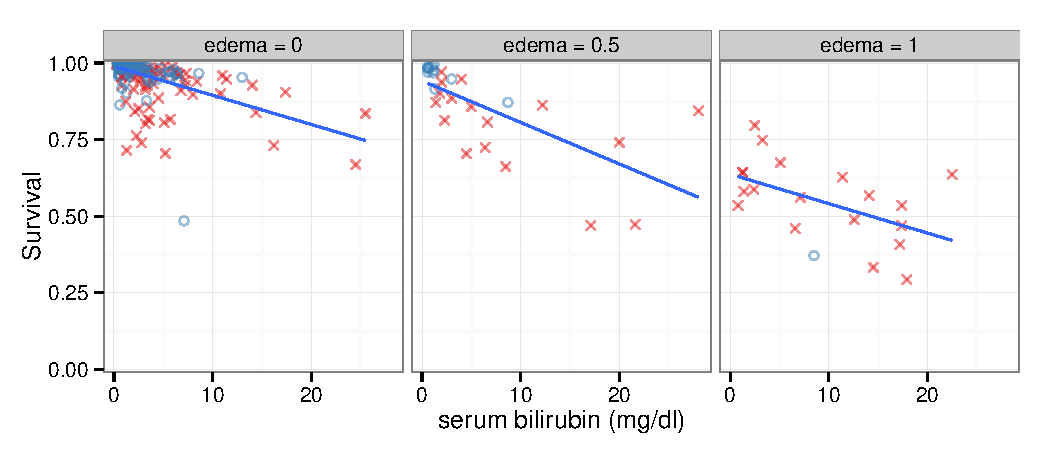
\includegraphics[width=\maxwidth]{figure/rfs-coplot_bilirubin-1} 

}

\caption[Variable dependence coplot]{Variable dependence coplot. Survival at 1 year against bilirubin, stratified by treatment and histological stage.\label{fig:coplot_bilirubin}}
\end{figure}
\end{Schunk}

Conditional membership with a continuous variable requires stratification at some level. Often we can make these stratification along some feature of the variable, for instance a variable with integer values, or 5 or 10 year age group cohorts. However in the variables of interest in our example, we have no "logical" stratification indications. Therefore we will arbitrarily stratify our variables into 6 groups of roughly equal population size using the \code{quantile_cuts} function. We pass the break points located by \code{quantile_cuts} to the \code{cut} function to create grouping intervals, which we can then add to the \code{gg_variable} object before plotting with the \code{plot.gg_variable} function. The simple modification to convert variable dependence plots into condition variable dependence plots is to use the \code{ggplot2::facet_wrap} command to generate a panel for each grouping interval.

\begin{Schunk}
\begin{Sinput}
R> copper_cts <- quantile_cuts(ggvar$copper, groups = 6)
R> copper_grp <- cut(ggvar$copper, breaks = copper_cts)
R> ggvar$copper_grp <- copper_grp
R> levels(ggvar$copper_grp) <- paste("copper = ",levels(copper_grp), sep = "")
R> 
R> plot(ggvar[-which(is.na(ggvar$copper)),], xvar = "bili", 
+                 method = "glm", alpha = .5, se = FALSE) + 
+   labs(y = "Survival", x = st.labs["bili"]) + 
+   theme(legend.position = "none") + 
+   scale_color_manual(values = strCol, labels = event.labels) + 
+   scale_shape_manual(values = event.marks, labels = event.labels)+ 
+   facet_wrap(~copper_grp)+
+   coord_cartesian(y = c(-.01,1.01))
\end{Sinput}
\begin{figure}[!htpb]

{\centering 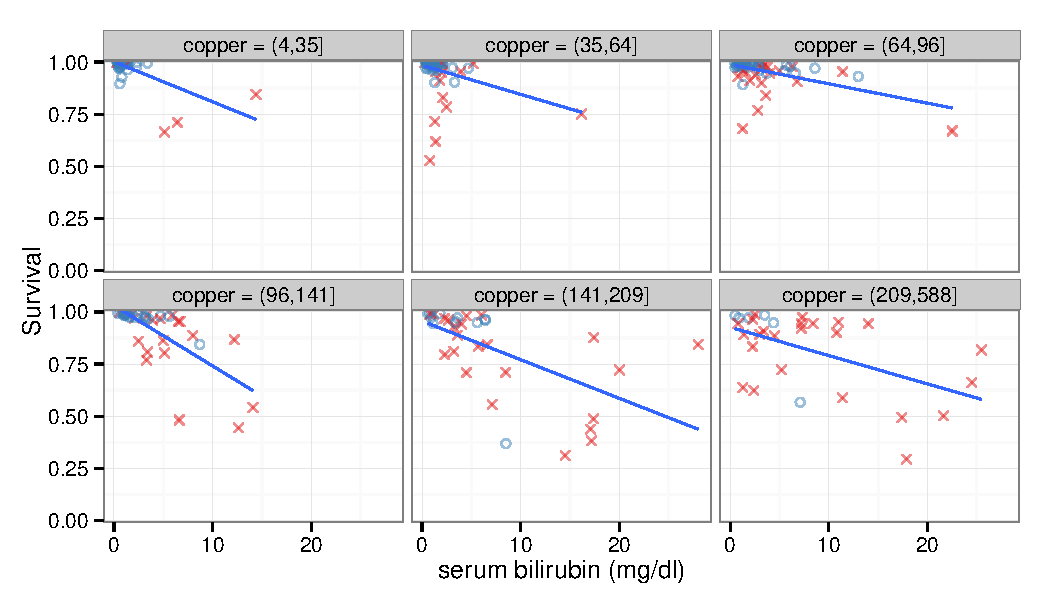
\includegraphics[width=\maxwidth]{figure/rfs-copper-coplot-1} 

}

\caption[Variable dependence coplot]{Variable dependence coplot. Survival at 1 year against bilirubin, stratified by conditonal membership in Urine Copper measurement intervalse.\label{fig:copper-coplot}}
\end{figure}
\end{Schunk}

To get a better feel for how the response depends on both variables, it is instructive to look at the complement coplot. We repeat the previous coplot process, predicted survival as a function of the \code{copper} variable, conditional on membership within 6 groups \code{bili} intervals. 


\begin{Schunk}
\begin{Sinput}
R> bili_cts <- quantile_cuts(ggvar$bili, groups = 6)
R> bili_grp <- cut(ggvar$bili, breaks = bili_cts)
R> ggvar$bili_grp <- bili_grp
R> levels(ggvar$bili_grp) <- paste("bilirubin = ",levels(bili_grp), sep = "")
R> 
R> plot(ggvar[-which(is.na(ggvar$copper)),], xvar = "copper", 
+                 method = "glm", alpha = .5, se = FALSE) + 
+   labs(y = "Survival", x = st.labs["copper"]) + 
+   theme(legend.position = "none") + 
+   scale_color_manual(values = strCol, labels = event.labels) + 
+   scale_shape_manual(values = event.marks, labels = event.labels)+ 
+   facet_wrap(~bili_grp)+
+   coord_cartesian(y = c(-.01,1.01))
\end{Sinput}
\begin{figure}[!htpb]

{\centering 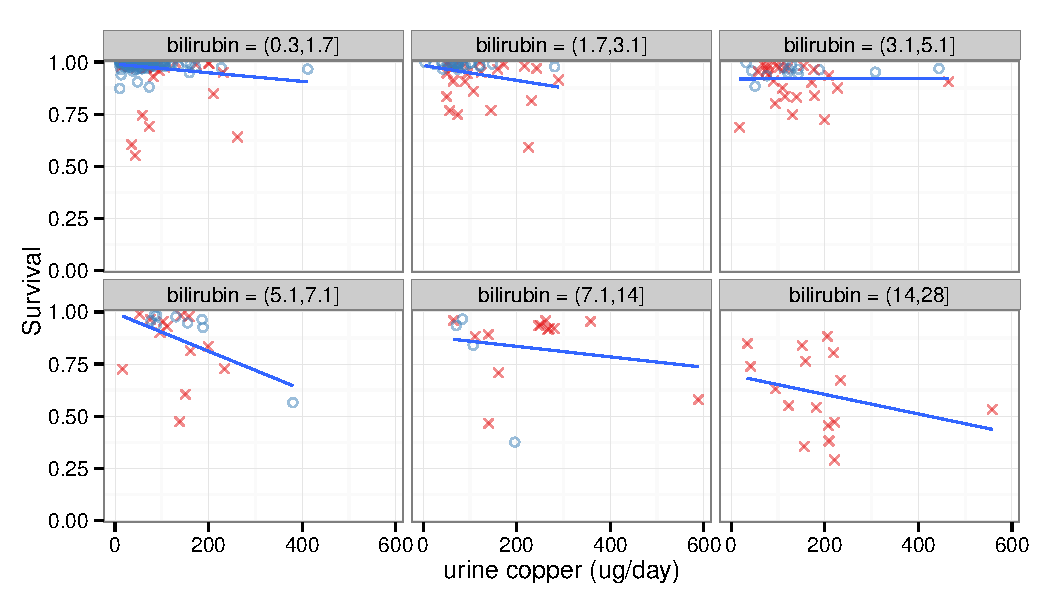
\includegraphics[width=\maxwidth]{figure/rfs-bili-coplot-1} 

}

\caption[Variable dependence coplot]{Variable dependence coplot. Survival at 1 year against bilirubin, stratified by conditonal membership in Urine Copper measurement intervalse.\label{fig:bili-coplot}}
\end{figure}
\end{Schunk}


We get similar information from this view,  However viewed together we get a better sense of how the  variables work together (interact) in the median value prediction.

Note that typically \cite{cleveland:1993} conditional plots for continuous variables included overlapping intervals along the grouped variable. We chose to use mutually exclusive continuous variable intervals for multiple reasons:
 \begin{itemize}
 \item Simplicity - We can create the coplot figures directly from the \code{gg_variable} object by adding a conditional group column directly to the object.

 \item Interpretability - We find it easier to interpret and compare the panels if each observation is only in a single panel.

 \item Clarity - We prefer using more space for the data portion of the figures than typically displayed in the \code{coplot} function available in base R, which require the bar plot to present the overlapping segments.
 \end{itemize}
 
It is still possible to augment the \code{gg_variable} to include overlapping conditional membership with continuous variables by duplicating rows of the object, and setting the correct conditional group membership. The \code{plot.gg_variable} function recipe above could then be used to generate the panel plot, with panels ordered according to the factor levels of the grouping variable. We leave this as an exercise for the reader.

\section{Partial dependence coplots}\label{partialcoplots}

By characterizing conditional plots as stratified variable dependence plots, the next logical step would be to generate an analogous conditional partial dependence plot. The process is similar to variable dependence coplots, first determine conditional group membership, then calculate the partial dependence estimates on each subgroup using the \code{randomForestSRC::plot.variable} function with a the \code{subset} argument for each grouped interval. The \code{gg_partial_coplot} function is a wrapper for generating a conditional partial dependence data object. Given a random forest (\code{randomForestSRC::rfsrc} object) and a \code{groups} vector for conditioning the training data set observations, \code{gg_partial_coplot} calls the \code{randomForestSRC::plot.variable} function for a set of training set observations conditional on \code{groups} membership. The function returns a \code{gg_partial_coplot} object, a sub class of the \code{gg_partial} object, which can be plotted with the \code{plot.gg_partial} function.

The following code block will generate the data object for creating partial dependence coplot of the predicted median home value as a function of \code{bili} conditional on membership within the 6 groups of \code{copper} ``intervals'' that we examined in the previous section.




Since the \code{gg_partial_coplot} makes a call to \code{randomForestSRC::plot.variable} for each group (6) in the conditioning set, we again resort to the data caching strategy, and load the stored result data from the \pkg{ggRandomForests} package. We modify the legend label to indicate we're working with groups of the , and use the \code{palette = "Set2"} Color Brewer(\url{http://colorbrewer2.org/}) color palette to choose a nice color theme for displaying the six curves.

\begin{Schunk}
\begin{Sinput}
R> data(partial_coplot_pbc, package = "ggRandomForests")
R> # Partial coplot
R> plot(partial_coplot_pbc, se = FALSE)+
+   labs(x = st.labs["bili"], y = "Survival at 1 year (%)", 
+        color = "Urine Copper", shape = "Urine Copper")+
+   scale_color_brewer(palette = "Set2")+
+   coord_cartesian(y = c(49,101))
\end{Sinput}
\begin{figure}[!htpb]

{\centering 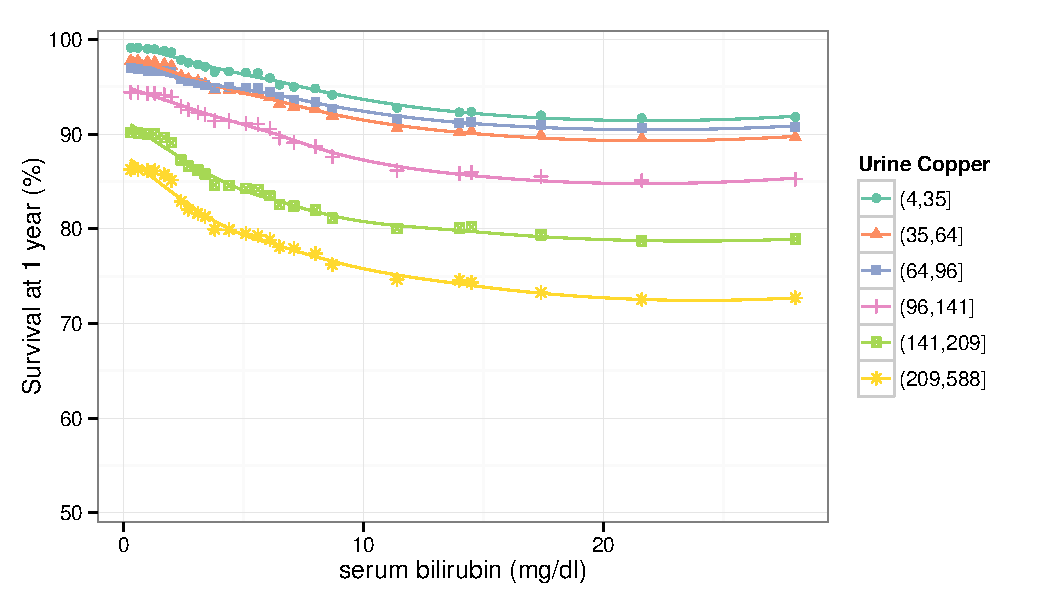
\includegraphics[width=\maxwidth]{figure/rfs-bili-copper-1} 

}

\caption[Partial (risk adjusted) variable dependence coplot]{Partial (risk adjusted) variable dependence coplot. Survival at 1 year against bilirubin, stratified by copper groups. Points mark risk adjusted estimates, loess smooth indicates predicted trend within each age group as a function of bilirubin.\label{fig:bili-copper}}
\end{figure}
\end{Schunk}

Unlike variable dependence coplots, we do not need to use a panel format for partial dependence coplots because we are looking risk adjusted estimates (points) instead of population estimates. 


We can view the partial coplot curves as slices along a surface viewed into the page, either along increasing or decreasing values. This is made more difficult by our choice to select groups of similar population size, as the curves are not evenly spaced along the `rm` variable. We return to this problem in the next section. 

We also construct the complement view, for partial dependence coplot of the  "intervals", and cache the following \code{gg_partial_coplot} data call.



\begin{Schunk}
\begin{Sinput}
R> data(partial_coplot_pbc2, package = "ggRandomForests")
R> # Partial coplot
R> plot(partial_coplot_pbc2, se = FALSE)+
+   labs(x = st.labs["copper"], y = "Survival at 1 year (%)", 
+        color = "Bilirubin", shape = "Bilirubin")+
+   scale_color_brewer(palette = "Set2")+
+   coord_cartesian(y = c(49,101))
\end{Sinput}
\begin{figure}[!htpb]

{\centering 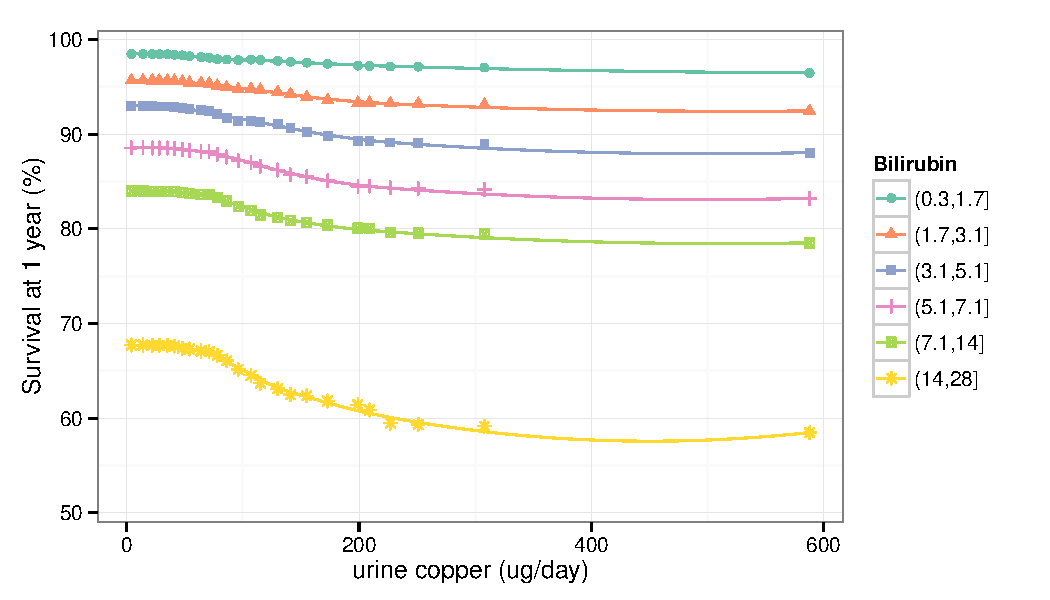
\includegraphics[width=\maxwidth]{figure/rfs-copper-bili-1} 

}

\caption[Partial (risk adjusted) variable dependence coplot]{Partial (risk adjusted) variable dependence coplot. Survival at 1 year against bilirubin, stratified by copper groups. Points mark risk adjusted estimates, loess smooth indicates predicted trend within each age group as a function of bilirubin.\label{fig:copper-bili}}
\end{figure}
\end{Schunk}

\section{Partial Plot Surfaces}

Visualizing two dimensional projections of three dimensional data is difficult, though there are tools available to make the data more understandable. To make the interplay of lower status and average room size a bit more understandable, we will generate a contour plot of the median home values. We could generate this figure with the data we already have, but the resolution would be a bit strange. To generate the plot of \code{bili} conditional on \code{copper} groupings, we would end up with contours over a grid of \code{bili} = $25 \times$ \code{copper} = $6$, for the alternative \code{copper} conditional on \code{bili} groups, we'd have the transpose grid of \code{bili} = $6 \times$  \code{copper} = $25$. 

Since we are already using the data caching strategy, we will generate another \code{gg_partial_coplot} data set with increased resolution in both the \code{bili} and \code{copper} dimensions. For this exercise, we will create 50 \code{copper} groups and generate the partial plot data at \code{npts = 50} points along the \code{bili} dimension for each group within the \code{plot.variable} call. This code block generates the 50 \code{copper} groups, each containing about 9 observations.     



We use the following data call to generate the \code{gg_partial_coplot} data object. This took about 15 minutes to run on a quad core Mac Air.



The cached \code{gg_partial_coplot} data object is included as a data set in the \pkg{ggRandomForests} package. We load the data, attach numeric values for the \code{copper} groups, and generate the figure.

\begin{Schunk}
\begin{figure}[!htpb]

{\centering \includegraphics[width=\maxwidth]{figure/rfs-contour3d-1} 

}

\caption[Partial coplot contour plot]{Partial coplot contour plot.\label{fig:contour3d}}
\end{figure}
\end{Schunk}

The contours are generated over the raw \code{gg_partial} estimation points, not smooth curves as shown in the partial plot and coplot figures. We can also generate a surface with this data using the \pkg{plot3D} \url{http://CRAN.R-project.org/package = plot3D} package and the \code{plot3D::surf3D} function. Viewed in 3D, a surface can help to better understand what the contour lines mean. 

\begin{Schunk}
\begin{figure}[!htpb]

{\centering 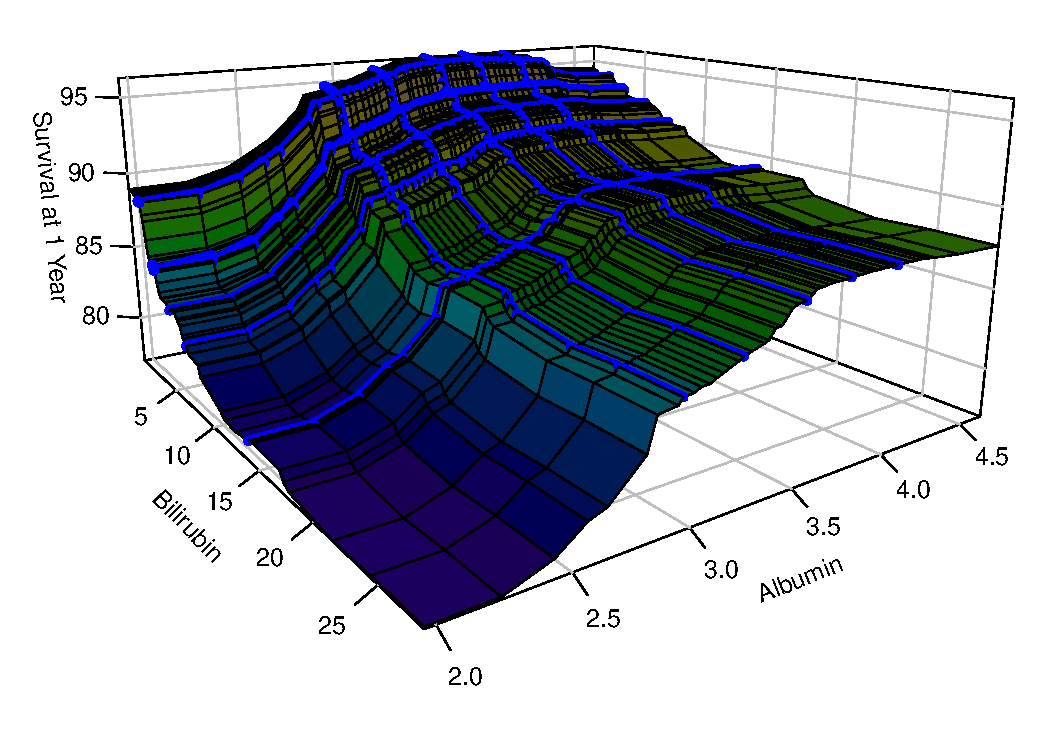
\includegraphics[width=\maxwidth]{figure/rfs-surface3d-1} 

}

\caption[Partial coplot surface]{Partial coplot surface.\label{fig:surface3d}}
\end{figure}
\end{Schunk}
%' 
%' 
%' 
%' <<def-pts2>>= 
%' # Find the quantile points to create 30 interval groups
%' bili_cts <- quantile_cuts(rfsrc_pbc$xvar$bili, groups = 49)
%' @
%' 
%' We use the following data call to generate the \code{gg_partial_coplot} data object. This took about 15 minutes to run on a quad core Mac Air.
%' 
%' <<prtl-surface2, eval=FALSE>>= 
%' # Generate the gg_partial_coplot data object
%' system.time(partial_pbc_surf2 <- lapply(bili_cts, function(ct){
%'   rfsrc_pbc$xvar$bili <- ct
%'   plot.variable(rfsrc_pbc, xvar = "copper", time = 1,
%'                 npts = 50, show.plots = FALSE, 
%'                 partial = TRUE, surv.type="surv")
%'   }))
%' #     user   system  elapsed 
%' # 2393.754   67.989 2465.498 
%' @
%' 
%' The cached \code{gg_partial_coplot} data object is included as a data set in the \pkg{ggRandomForests} package. We load the data, attach numeric values for the \code{copper} groups, and generate the figure.
%' 
%' <<contour3d2, fig.cap="Partial coplot contour plot.", fig.width=7, fig.height=5>>= 
%' # Load the stored partial coplot data.
%' data(partial_pbc_surf2)
%' 
%' # Instead of groups, we want the raw rm point values,
%' # To make the dimensions match, we need to repeat the values
%' # for each of the 50 points in the lstat direction
%' bili.tmp <- do.call(c,lapply(bili_cts, 
%'                                function(grp){rep(grp, 50)}))
%' 
%' # Convert the list of plot.variable output to 
%' partial_surf2 <- do.call(rbind,lapply(partial_pbc_surf2, gg_partial))
%' 
%' # attach the data to the gg_partial_coplot
%' partial_surf2$bili <- bili.tmp
%' 
%' # ggplot2 contour plot of x, y and z data.
%' ggplot(partial_surf2, aes(x = bili, y = copper, z = yhat))+
%'   stat_contour(aes(colour = ..level..), binwidth = .25)+
%'   labs(x = st.labs["bili"], y = st.labs["copper"], 
%'        color = "Survival at 1 year (%)")+
%'   scale_colour_gradientn(colours = topo.colors(25))
%' @
%' 
%' The contours are generated over the raw \code{gg_partial} estimation points, not smooth curves as shown in the partial plot and coplot figures. We can also generate a surface with this data using the \pkg{plot3D} \url{http://CRAN.R-project.org/package = plot3D} package and the \code{plot3D::surf3D} function. Viewed in 3D, a surface can help to better understand what the contour lines mean. 
%' 
%' <<surface3d2, fig.cap="Partial coplot surface.", fig.width=7, fig.height=5>>= 
%' # Modify the figure margins to make the figure larger
%' 
%' par(mai = c(0,0,0,0))
%' 
%' # Transform the gg_partial_coplot object into a list of three named matrices
%' # for surface plotting with plot3D::surf3D
%' srf <- surface_matrix(partial_surf2, c("bili", "copper", "yhat"))
%' 
%' # Generate the figure.
%' surf3D(x = srf$x, y = srf$y, z = srf$z, col = topo.colors(25),
%'        colkey = FALSE, border = "black", bty = "b2", 
%'        shade = 0.5, expand = 0.5, 
%'        lighting = TRUE, lphi = -50,
%'        xlab = "Bilirubin", ylab = "Urine Copper", zlab = "Survival at 1 Year"
%' )
%' @

\section{Time Dimension}






The cached \code{gg_partial_coplot} data object is included as a data set in the \pkg{ggRandomForests} package. We load the data, attach numeric values for the \code{copper} groups, and generate the figure.

\begin{Schunk}
\begin{figure}[!htpb]

{\centering \includegraphics[width=\maxwidth]{figure/rfs-timeContour3D-1} 

}

\caption[Partial coplot contour plot]{Partial coplot contour plot.\label{fig:timeContour3D}}
\end{figure}
\end{Schunk}

The contours are generated over the raw \code{gg_partial} estimation points, not smooth curves as shown in the partial plot and coplot figures. We can also generate a surface with this data using the \pkg{plot3D} \url{http://CRAN.R-project.org/package = plot3D} package and the \code{plot3D::surf3D} function. Viewed in 3D, a surface can help to better understand what the contour lines mean. 

\begin{Schunk}
\begin{figure}[!htpb]

{\centering 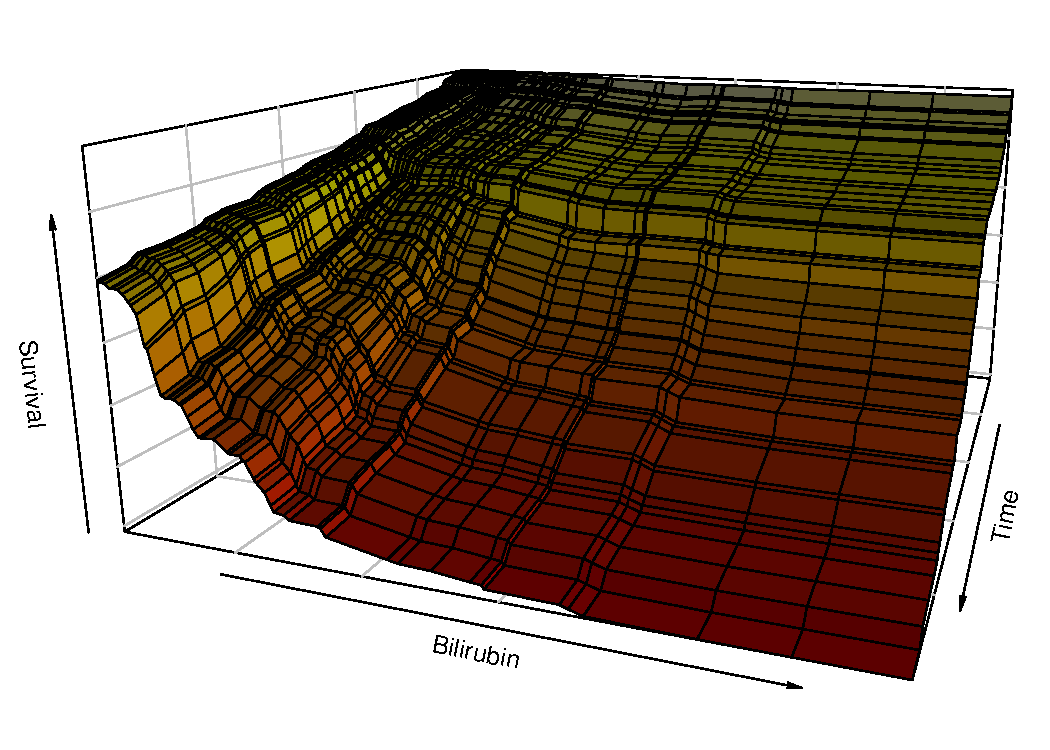
\includegraphics[width=\maxwidth]{figure/rfs-timeSurface3d-1} 

}

\caption[Partial coplot surface]{Partial coplot surface.\label{fig:timeSurface3d}}
\end{figure}
\end{Schunk}

\section{Conclusion}

\appendix

%\singlespacing
\bibliography{ggRandomForests}

\end{document}


---


\subsection{ggRandomForests}
The \pkg{randomForestSRC} package is a mature analysis and research random forest implementation under rapid development. The package includes diagnostic and post processing functions for analysis and visualizations of randomForest model properties. However, in our research we frequently found it difficult to manipulate the standard figures directly produced with the \pkg{randomForestSRC} package. 

In order to simplify these manipulations, we developed the \pkg{ggRandomForests} package. We attempted to follow two design principles in this development:
\begin{itemize}
\item Model/View separation: The package originally designed to generating \pkg{ggplot2}~\cite{Wickham:2009} figures for random forest objects. However, some users would prefer to use other graphing methods within \proglang{R} or outside of it. To help users, we separate the data generation and the figure generation into two separate operations. 

\item Modular: We strive to create a modular design by following the \emph{do one thing well} philosphy. Each function operates on one \pkg{randomForestSRC} object to create only one data object or figure type.
\end{itemize}
